\documentclass[10pt,a4paper,reqno]{amsart}


\textwidth=16.5cm
\textheight=20cm%21.5cm
\oddsidemargin=0cm
\evensidemargin=0cm

\usepackage[sort&compress]{natbib}
\usepackage{lipsum}

\usepackage{amssymb,amsmath,bm,mathrsfs}
\usepackage{graphicx}
\usepackage{enumerate}
%\usepackage[notcite]{showkeys}
%\usepackage{color}
%\usepackage{showlabels}
%\renewcommand{\showlabelfont}{\small\slshape\color{red}}

\usepackage{lineno}
\linenumbers

\usepackage{amsthm}
\usepackage{mathabx}
%\usepackage{hyperref} %$#

%%%%%%%%%%%%%%%%%

%Math environments===========================================================
\newtheorem{theorem}{Theorem}[section]
\newtheorem{lemma}[theorem]{Lemma}
\theoremstyle{definition}
\newtheorem{definition}[theorem]{Definition}
\newtheorem{example}[theorem]{Example}
\newtheorem{xca}[theorem]{Exercise}
\newtheorem{corollary}[theorem]{Corollary}
\newtheorem{proposition}[theorem]{Proposition}
\newtheorem{assumption}[theorem]{Assumption}
\theoremstyle{remark}
\newtheorem{remark}[theorem]{Remark}
\renewcommand{\labelenumi}{\roman{enumi})}
\numberwithin{equation}{section}

\font\name=cmr8

\newcommand {\rank}     {\mathop{\rm rank}\nolimits}
\newcommand {\corank}   {\mathop{\rm corank}\nolimits}
\newcommand {\range}  {\mathop{\rm range}\nolimits}
\newcommand {\corange}  {\mathop{\rm corange}\nolimits}
\newcommand {\kernel}   {\mathop{\rm kernel}\nolimits}
\newcommand {\cokernel} {\mathop{\rm cokernel}\nolimits}
\newcommand {\basis}    {\mathop{\rm basis}\nolimits}
\newcommand {\sigmin}   {\mathop{\sigma_{\rm min}}\nolimits}
\newcommand {\ind}      {\mathop{\rm ind}\nolimits}
\newcommand {\opt}      {\mathop{\rm opt}\nolimits}
\newcommand{\diag}{\mbox{\rm diag}}
\newcommand{\upt}{\mbox{\rm up}}
\newcommand{\re}{\mbox{\rm Re}}
\newcommand{\im}{\mbox{\rm Im}}
\newcommand{\dps}{\displaystyle}
\newcommand{\sct} {{\,\stackrel{c}{\sim}\,}}
\newcommand{\sue} {\,{\stackrel{u}{\sim}\,}}
\newcommand{\suc} {\,{\stackrel{uc}{\sim}\,}}
%\renewcommand{\comment}[1]{}
%\renewcommand{\proof}{\par\noindent{\bf Proof}. \ignorespaces}
%\newcommand{\eproof}{\space
%	{\ \vbox{\hrule\hbox{\vrule height1.3ex\hskip0.8ex\vrule}\hrule}} \ignorespaces} %\\[0.2cm]}
%
%=======================================================================================
% new def-s and commands
%\include{HaMe12_Feb18_command}

\def\bbI{\mathbb{I}}
\def\bbL{\mathbb{L}}
\def\bbM{\mathbb{M}}

\def\om{\omega}
\def\leq{\leqslant}
\def\rar{\rightarrow}
\def\Rar{\Rightarrow}
\def\td{\Leftrightarrow}
\def\r{\hro{R}}
\def\C{\hro{C}}
\def\hro{\mathbb}
\def\N{\hro{N}}

\def\a{\alpha}
\def\b{\beta}
\def\B{\mathcal B}
\def\lb{\lambda}
\def\Lb{\Lambda}
\def\vphi{\varphi}
\def\de{\delta}
\def\De{\Delta}
\def\ga{\gamma}
\def\Si{\Sigma}
\def\si{\sigma}
\def\ka{\kappa}
\def\tka{\tilde{\kappa}}
\def\CE{\mathcal{E}}
\def\tE{\tilde{E}}
\def\hE{\hat{E}}
\def\tA{\tilde{A}}
\def\hA{\hat{A}}
\def\bA{\breve{A}}
\def\tB{\tilde{B}}
\def\tD{\tilde{D}}
\def\hB{\hat{B}}
\def\hr{\hat{r}}
\def\hv{\hat{v}}
\def\tr{\tilde{r}}
\def\trho{\tilde{\rho}}

\def\nab{\nabla}

\def\cB{\mathcal B}
\def\cM{\mathcal M}
\def\tcM{\tilde{\mathcal M}}
\def\cN{\mathcal N}
\def\cX{\mathcal X}
\def\cS{\mathcal S}
\def\tU{\tilde{U}}
\def\cU{\mathcal U}
\def\cL{\mathcal L}

\def\tN{\tilde{N}}
\def\hN{\hat{N}}
\def\tk{\tilde{k}}
\def\hk{\hat{k}}
\def\tx{\tilde{x}}
\def\tX{\tilde{X}}
\def\hX{\hat{X}}
\def\tY{\tilde{Y}}
\def\hY{\hat{Y}}
\def\ty{\tilde{y}}
\def\tv{\tilde{v}}
\def\tw{\tilde{w}}

\def\tM{\tilde{M}}
\def\tm{\tilde{m}}
\def\bM{\breve{M}}
\def\hM{\hat{M}}
\def\bm{\breve{m}}

\def\tC{\tilde{C}}
\def\hC{\hat{C}}
\def\hD{\hat{D}}

\def\tH{\tilde{H}}
\def\tF{\tilde{F}}
\def\tG{\tilde{G}}
\def\hG{\hat{G}}
\def\cG{{\cal G}}
\def\baf{\bar{f}}
\def\tg{\tilde{g}}
\def\hg{\hat{g}}
\def\tK{\tilde{K}}

\def\cW{{\cal W}}

\def\tS{\tilde{S}}
\def\tZ{\tilde{Z}}

\def\tx{\tilde{x}}
\def\tf{\tilde{f}}
\def\hf{\hat{f}}
\def\brf{\breve{f}}
\def\bX{\breve{X}}

\def\chA{\widecheck{A}}
\def\chB{\widecheck{B}}
\def\chC{\widecheck{C}}
\def\chD{\widecheck{D}}
\def\chG{\widecheck{G}}
\def\chU{\widecheck{U}}

\def\lsim{\overset{\ell}{\sim}}
% The inverse shift operator
\def\ide{\Delta_{-1}}


\def\be{\begin{equation}}
\def\ee{\end{equation}}         

\newcommand{\ben}{\begin{eqnarray}}
\newcommand{\een}{\end{eqnarray}}

\newcommand{\bsen}{\begin{subeqnarray}}
\newcommand{\esen}{\end{subeqnarray}}

\newcommand{\bens}{\begin{eqnarray*}}
\newcommand{\eens}{\end{eqnarray*}}

\def\bc{\begin{cases}}
\def\ec{\end{cases}}

\newcommand{\bsq}{\begin{subequations}}
\newcommand{\esq}{\end{subequations}}

\newcommand{\m}[1]{
	\begin{bmatrix}
		#1 
	\end{bmatrix}
}

\renewcommand{\pm}[1]{
	\begin{matrix}
		#1 
	\end{matrix}
}

\newcommand{\n}[1]{
	\|	#1 \|
}

\def\Px{P_{\mathrm{x}}}
\def\Py{P_{\mathrm{y}}}

\def\BEA{\cB^{EA}(\r_+,\r^n)}
%===============================================================================
\begin{document}
	

\title[EXPONENTIAL DICHOTOMY AND STABLE MANIFOLD FOR DAEs]{EXPONENTIAL DICHOTOMY AND STABLE MANIFOLDS FOR DIFFERENTIAL-ALGEBRAIC EQUATIONS ON THE HALF-LINE}

\author[N.T. Huy]{Nguyen Thieu Huy}
\address{Nguyen Thieu Huy, School of Applied Mathematics and Informatics,
	Hanoi University of Science and Technology,
	Vien Toan ung dung va Tin hoc, Dai hoc Bach khoa Ha Noi,
	1 Dai Co Viet, Hanoi, Vietnam}
\email{huy.nguyenthieu@hust.edu.vn}

\author[H. Phi]{Ha Phi}
\address{Ha Phi,  Faculty of Mathematics-Mechanics-Informatics, Hanoi University of Science,
	Khoa Toan-Co-Tin hoc, Dai Hoc Khoa Hoc Tu Nhien, DHQGHN,
	334 Nguyen Trai St., Hanoi, Vietnam}
\email{haphi.hus@vnu.edu.vn}


\begin{abstract}
We study linear and semi-linear differential-algebraic equations (DAEs) on the half-line $\r_+$. 
Firstly, we characterize the existence of exponential dichotomy for linear DAEs based on the Lyapunov-Perron method. Then, we prove the existence of local and global, invariant, stable manifolds for semi-linear DAEs in the case that the  evolution family corresponding to linear DAE admits an exponential dichotomy and the nonlinear forcing function fulfills the non-uniform $\vphi$-Lipschitz condition, in which the Lipschitz function $\vphi$ belongs to wide classes of admissible function spaces such as $L_p$, $1\leq p \leq \infty$, $L_{p,q}$, etc.  
\end{abstract}
\keywords{Exponential dichotomy, semilinear, differential-algebraic equation, admissibility of function spaces, stable manifold.}
\maketitle

%\baselineskip= .6cm

%%%%%%%%%%%%%%%%%%%%%%%%%%%%%%%  Section 1
%%%%%%%%%%%%%%%%%%%%%%%%%%%%%%%%%%
\section{Introduction and Preliminaries} \label{section 1}
 The present paper  focuses on the existence of invariant 
(local and global) stable manifolds for semi-linear non-autonomous differential-algebraic equations (DAEs) of the form
%
\begin{equation}\label{eq1}
\pm{d \mbox{ rows }\\ a \mbox{ rows }} \quad \underbrace{\m{E_1(t) \\ 0}}_{E(t)}  \dot{x}(t) = \underbrace{ \m{A_1(t) \\ A_2(t)} }_{A(t)} x(t) + 
\underbrace{ \m{f_1(t,x(t)) \\ f_2(t,x(t))} }_{f(t,x(t))} , \quad t\in \r_+:=[0,+\infty).
\end{equation}
%
To do that, we start by investigating 
the exponential dichotomy of the associated linear system
%
\begin{equation}\label{eq2}
E(t)\dot{x}(t) = A(t) x(t), \quad t\in [0,+\infty).
\end{equation}
%
Here $E=\m{E_1(t) \\ 0}$, $A = \m{A_1(t) \\ A_2(t)}$ are assumed to be matrix-valued functions acting 
on $\r_+$ to $\r^{n,n}$, 
$x: \r_+  \rightarrow \r^{n}$, $f:\r_+ \times \r{^n} \rightarrow \r{^n}$. Furthermore, we assume that for all $t$, the matrices $E_1(t)$, $A_2(t)$ have full row rank. 

DAE systems of the forms \eqref{eq1}, \eqref{eq2} arise in many applications, include multibody dynamics, electrical circuits, chemical engineering, and many other applications. 
Due to the rank-deficiency of $E(t)$, the qualitative behavior of DAEs is much richer, in comparison to ordinary differential equations (ODEs). We refer the reader to recent monographs \cite{BieCM12,KunM06,LamMT13,IlcR13} and the references therein. 
In particular, even though the stability analysis for DAEs have been intensively discussed (see the survey \cite[Chapter 2]{IlcR13}), 
there are only few papers on the spectral theory of DAEs and in particular, the exponential dichotomy for DAEs. 
We refer to \cite{LenM90} for the concept of exponential dichotomy and its relation to the well conditioning of the associated boundary value problem, to \cite{LinM09} for Lyapunov and other spectra for linear DAEs, to \cite{ChyDL08,DuL06} for the robustness of exponential stability and Bohl exponents. 

On the other hand, whenever the exponential dichotomy of the linear, homogeneous system \eqref{eq2} is characterized, 
the next important question in the qualitative theory of DAEs is to study the existence of  integral manifolds (e.g., stable, unstable, center, center-stable, center-unstable) for the semi-linear DAE \eqref{eq1} \cite{DalK02,Chi13}. 
Unfortunately, till now this question is essentially open for DAEs. In order to shorten these gaps, this paper is devoted to investigation of
 the exponential dichotomy of \eqref{eq2} and stable manifolds of \eqref{eq1}. Our method is based on the classical "Lyapunov-Perron method" (\cite{DalK02,Zhi72}) and the admissibility of function spaces (\cite{Huy06,Huy09a}). 

The outline of this paper is as follows. In the rest of this first section we recall some basis concepts for later use, including the notion of the exponential dichotomy and its properties, as well as some important features of admissible function spaces. 
%Then, in Section \ref{Sec 2} we present the admissibility of function spaces and their properties. 
 In Section \ref{Sec 3} we gives a characterization for the existence of exponential dichotomy for the DAE \eqref{eq2}. 
Section \ref{Sec 4} contains our main results on the existence and properties of local stable manifold for the semi-linear DAE \eqref{eq1}. The global version of these results will be presented in Section \ref{Sec 5}. Finally, we illustrate our results by studying a spatial discretization of  Navier-Stokes equations, and we conclude this research by a summary and some open problems.\\

\subsection{Evolution Families and Exponential Dichotomies}
Let us now recall some basic notions. By ($\r^n$, $\n{\cdot}$) we denote the n-dimensional real vector space equipped with the Euclidean norm. For any matrix $V$, by $V^T$ we denote its transpose. \ 
For any $p\in \N$, by $C^p([0,\infty),\r^n)$ we denote the space of $p$-times continuously differentiable functions acting on $[0,\infty)$ with values in $\r^n$. 
By $C_{b}([0,\infty),\r^n)$ we denote the space of continuous and bounded functions mapping from $[0,\infty)$ into $\r^n$. 
This space is a Banach space with the $ess\sup$-norm $\|f\|_{\infty}:=\sup\{\|f(t)\|, \ t \geq 0\}$. 
%\ By $L_{\infty}(\r_+,\r^n)$ we denote the space of locally integrable functions that is essentially bounded, i.e. 


It is well-known (e.g. \cite{Chi13}), that for ordinary differential equations (ODEs), if the Cauchy problem
%
\begin{align}\label{eq3}
\dfrac{dx(t)}{dt} &= A(t)x(t), \ t\geq s \geq 0,\\
			x(s)  &= x_s \in \r^{n}, \notag 
\end{align}
%
is well-posed, then there exists a pointwise nonsingular matrix-valued function $(t,s)\mapsto X(t,s)\in \r^{n,n}$ such that the solution of $\eqref{eq3}$ is given by  $x(t)=X(t,s)x_s$.
This fact motivates the existence of an evolution family $(X(t,s))_{t\geq s\geq 0}$ associated with the matrix function $A(t)$.
This family satisfies the condition $X(t,t)=Id$ and the so-called \emph{semi-group property}
%
\begin{equation}\label{semigroup prop}
X(t,r)X(r,s) = X(t,s), \mbox{ for all } t\geq r\geq s\geq 0.
\end{equation}
%
Furthermore, the solution of the corresponding semi-linear ODE
%
%\be\label{semilinear ODE}
\[ \dfrac{dx(t)}{dt} = A(t)x(t) + f(t,x(t)), \ \mbox{ for all }t\geq s \geq 0,
\]
%\ee
%
is given by the so-called \emph{variation-of-constant formula}
%
\be\label{variational form}
x(t) = X(t,s)x(s) + \int_s^t X(t,\tau) f(\tau,x(\tau)) d\tau, \ \mbox{ for all }t\geq s \geq 0.
\ee
%
%The concept of an evolution family has been extended for abstract ODEs as follows.
%%
%\begin{definition}\label{def1} (\cite{Chi13})
%	A family of operators  $\{X(t,s)\}_{t\geq s\geq 0}$\quad  acting on a Banach space $\r^{n}$  is a (strongly continuous, exponential bounded) evolution family if
%	\begin{enumerate}
%		\item[(i)]  $X(t,t)=Id$ and $X(t,r)X(r,s) = X(t,s)$ for all $t\geq r\geq s\geq 0.$ 
%		\item[(ii)] The map $(t,s)\mapsto X(t,s)x$ is continuous for every $x\in\r^{n}$,
%		\item[(iii)]  $\|X(t,s)x\|\leq Ke^{c(t-s)}\|x\|$  for  all   $t\geq s\geq 0$
%		and  $x\in\r^{n}$,  for some constants  $K,c.$
%	\end{enumerate}
%\end{definition}
%%
%The notion of an evolution family arises naturally from the theory of evolution  equation which are well-posed. 
For more details on the notion and discussion on properties and applications of evolution families we refer the readers to Pazy \cite{Paz12}.
%
\begin{definition}\label{def2}
A given evolution family $\{X(t,s)\}_{t\geq s\geq 0}$ of the ODE \eqref{eq3} is said to have an \emph{exponential dichotomy} on the half-line if there exist a family of projection matrices $\{P(t)\}_{t\geq 0}$ and two positive constants $N,\nu$ such that the following conditions are satisfied.
\begin{enumerate}
	\item[i)] $P(t)(t)X(t,s)=X(t,s)P(s)$  for all  $t\geq s\geq 0$, 		
	\item[ii)] the restriction $X(t,s)_{|}: \ker P(s) \rar \ker P(t)$ is an isomorphism and we denote the inverse of $X(s,t)_{\mid}$, 
	\item[iii)] $\|X(t,s) P(s)x \| \leq Ne^{-\nu(t-s)}\|P(s)x\|$, for all $t\geq s \geq 0$, $x\in \r^n$, 
	\item[iv)]  $\|X(t,s)_| \ (I-P(s)) x \| \leq Ne^{\nu(t-s)}\| (I-P(s)) x\|$, for all $s\geq t \geq 0$, $x\in \r^n$.		
\end{enumerate}
Here $\{P(t)\}_{t\geq 0}$ (reps. $N$, $\nu$) are called \emph{dichotomy projections} (resp. \emph{dichotomy constants}).
\end{definition}

Next we recall some basic concepts and properties for DAEs, starting with \emph{fundamental solution matrix} as below.
%
\begin{definition}
	(i) Consider the DAE \eqref{eq2}. A matrix function $X \in C([0,\infty),\r^{n,k})$, $d\leq k \leq n$, is called \emph{a fundamental solution matrix} of \eqref{eq2} if each of its columns is a solution to \eqref{eq2} and $\rank X(t)=d$, for all $t\geq 0$. \\
	(ii) A fundamental solution matrix is said to be \emph{maximal} if $k=n$ and \emph{minimal} if $k=d$, respectively. A maximal fundamental solution is called \emph{principal} if it satisfies the \emph{projected initial condition}
	%
	\begin{equation}\label{projected intial condition}
	 E(0) \left( X(0) - Id \right) = 0.
	\end{equation}
	%
\end{definition}
%
We can easily see that, the fundamental solution matrices for DAEs are not necessarily square or of full rank. Furthermore, each fundamental solution matrix has exactly $d$-linear independent columns, and a minimal fundamental solution matrix can be made maximal by adding $n-d$ zero columns. This is the major difference between ODEs and DAEs. Consequently, we are unable to define the evolution family for a DAE in the classical sense. The modified concept, but still capture the essence of an original one, has been proposed and carefully discussed in \cite{LinM09}. We recall it below, and notice that this concept is equivalent to the one proposed by Lentini and M\"arz in \cite{LenM90} within the context of the matrix chains approach and tractability index.
Throughout this paper, we will assume the following.
%
\begin{assumption}\label{Ass1}
Consider the DAEs \eqref{eq1}, \eqref{eq2}. We assume that the function pair $(E,A)$ in these DAEs is \emph{strangeness-free}, i.e., 
%
\[
\rank \m{E_1(t) \\ A_2(t)} = n,
\]
%
for all $t\geq 0$. Furthermore, we assume that $E \in C^1([0,\infty),\r^{n,n})$ and $A \in C^0([0,\infty),\r^{n,n})$.
\end{assumption}
%
It should be important to note, that for general linear, homogeneous DAE of the form \eqref{eq2}, one can transform it to the strangeness-free form without alternating the solution space. For further details, see \cite[Chap. 3]{KunM06}.\\
%%
%\begin{lemma}\label{thm3.9KunM06}(\cite[Theorem 3.9]{KunM06})
%Let $E\in C^{\ell}(\hro{I},\C^{m,n})$, $\ell\in \N_0\cup \{\infty\}$, with constant $\rank E(t)=d$ for all $t\in \hro{I}$. Then there exist pointwise nonsingular
%functions $U\in C^{\ell}(\hro{I},\C^{m,m})$ and $V\in C^{\ell}(\hro{I},\C^{n,n})$, such that 
%%
%\[
%U^HEV= \m{\Si & 0 \\ 0 & 0},
%\]
%%
%with pointwise nonsingular $\Si \in C^{\ell}(\hro{I},\C^{d,d})$.
%\end{lemma}
%%
%\textbf{\large Need to write more about Moore-Penrose pseudo inverse for $E(t)$ to prepare for Section 3}

By making use of some smooth factorizations, for example QR or SVD (\cite{DieE99}  or \cite{KunM06}, Theorem 3.9), we can decouple and then exploit the structure of the DAE \eqref{eq2} in the following lemma.

%\begin{lemma}\label{lem0}
%	Consider the DAE \eqref{eq1} and assume that it satisfies Assumption \ref{Ass1}. \\
%	i) Then, there exists a continuous, pointwise-orthogonal matrix function $V(t)$, $t\geq 0$, such that by changing variable $x(t) = V(t)y(t)$, we can transform \eqref{eq1} to the form
%	%
%	\begin{equation}\label{decoupled system}
%	\m{\Si(t) & 0 \\ 0 & 0} \m{ \dot{y}_1(t) \\ \dot{y}_2(t)} = \m{\tA_1(t) & \tA_2(t) \\ \tA_3(t) & \tA_4(t)} \m{ y_1(t) \\ y_2(t)} + \m{\tf_1(t,y_1(t),y_2(t)) \\  \tf_2(t,y_1(t),y_2(t))},
%	\end{equation}
%	%
%	with pointwise nonsingular matrix functions $\Si(t) \in \r^{d,d}$ and $\tA_4(t) \in \r^{a,a}$. \\
%	ii) Consequently, the DAE \eqref{eq1} becomes the coupled system
%	%
%	\begin{align}\label{coupled system}
%	\label{decoupled system.1} \Si(t) \dot{y}_1(t) &=  \tA_1(t)y_1(t) + \tA_2(t)y_2(t) + \tf_1(t,y_1(t),y_2(t)), \\
%	\label{decoupled system.2} 0 &= \tA_3(t)y_1(t) + \tA_4(t)y_4(t) + \tf_2(t,y_1(t),y_2(t)).
%	\end{align}
%	%
%\end{lemma}

\begin{lemma}\label{lem1}
Consider the DAE \eqref{eq2} and assume that it satisfies Assumption \ref{Ass1}. Then, there exist  pointwise-orthogonal matrix-valued functions $U$ and $V\in C^1([0,\infty),\r^{n,n})$, such that after changing variable $x(t) = V(t)y(t)$, and scaling \eqref{eq2} with $U(t)$, we can transform it to the so-called \emph{decoupled system} of the following form
%
\be\label{decoupled system}
\m{\Si(t) & 0 \\ 0 & 0} \m{ \dot{y}_1(t) \\ \dot{y}_2(t)} = \m{\tA_1(t) & \tA_2(t) \\ \tA_3(t) & \tA_4(t)} \m{ y_1(t) \\ y_2(t)},
\ee
%
with pointwise nonsingular matrix-valued functions $\Si(t) \in \r^{d,d}$ and $\tA_4(t) \in \r^{a,a}$. 
%
\end{lemma}
\begin{proof} Applying an SVD factorization for $E_1(t)$ we can find 
pointwise-orthogonal matrix functions $U_1(t) \in C^1([0,\infty),\r^{d,d})$ and $V\in C^1([0,\infty),\r^{n,n})$	
such that
%
$ U_1(t) E_1(t) V(t) = \m{\Si(t) & 0}$,
%	  
where $\Si(t)$ is a continuous, pointwise nonsingular function with values in $\r^{d,d}$. Changing the variable $x(t) = V(t)y(t)$ and scaling \eqref{eq2} with $U(t):=\m{U_1(t) & 0 \\ 0 & I_{a}}$, we obtain a new system 
%
\[
U(t) E(t) V(t) y(t) = U(t) \left( A(t)V(t) - E(t)\dot{V}(t) \right) y(t),
\]
%
which is exactly of the form \eqref{decoupled system}. Furthermore, notice that 
%
\[
\m{\Si(t) & 0 \\ \tA_3(t) & \tA_4(t)} = \m{U_1(t) & 0 \\ 0 & I_{a}} \ \m{E_1(t) \\ A_2(t)} \ V,
\]
%
then Assumption \ref{Ass1} yields that both $\Si$ and $\tA_4$ are nonsingular. This completes the proof.
\end{proof}
%
Let $\hA_3 := -\tA^{-1}_4(t) \tA_3(t)$, $\hA_1 := \Si^{-1}(t) \tA_1(t) + \Si^{-1}(t) \tA_2(t) \tA^{-1}_4(t) \tA_3(t)$, we rewrite the transformed system \eqref{decoupled system} as
%
\begin{align}
\label{eq5.1} \dot{y}_1(t) &= \hA_1(t) y_1(t), \\ 
\label{eq5.2} y_2(t) &= \hA_3(t) y_1(t).
\end{align}
%
Since $V(t)$ is orthogonal for all $t\geq 0$, we see that all important qualitative properties of $x(t)$, such as boundedness, exponential stability, contractivity, expansiveness, etc., can be carried out for the function $y(t)$. Clearly, we see that \eqref{eq5.2} gives an \emph{algebraic constraint} that the solution to \eqref{decoupled system} must obey, while \eqref{eq5.1} gives the dynamic of \eqref{decoupled system}. 
For this reason, we call it \emph{an underlying ODE} to \eqref{decoupled system}.\\

Let $\{\hY_1(t,s)\}_{t\geq s \geq 0}$ be the evolution family associated with the matrix function $\hA_1(t)$, then we can define the corresponding evolution families for two DAEs \eqref{decoupled system}, \eqref{eq2} consecutively as follows.
%
\begin{equation}\label{eq4}
\hY(t,s) := \m{\hY_1(t,s) & 0 \\ \hA_3(t) \hY_1(t,s) & 0}, \ \hX(t,s) = V(t)\hY(t,s) V^T(s), \mbox{ for all } t\geq s \geq 0.
\end{equation}
%
Nevertheless, since $X(t,s)$ is not invertible, we will define the \emph{reflexive generalized inverse matrix function} as in \cite{LinM09} by 
%
\be\label{eq5}
\hY^-(t,s):= \m{\hY^{-1}_1(t,s) & 0 \\ \hA_3(s) \hY^{-1}_1(t,s) & 0} , \ \hX^-(t,s):= V(s) \hY^-(t,s) V^T(t), \mbox{ for all } t\geq s \geq 0.
\ee
% 
Furthermore, we can directly verify the semigroup properties, i.e.  
%
\begin{align*}
\hX(t,r) & = \hX(t,s) \hX(s,r), \mbox{ for all } t\geq s \geq r \geq 0, \\
\hX(t,s) & = \hX(t,0) \hX^-(s,0), \mbox{ for all } t\geq s \geq 0.
\end{align*}
%

Now we give a solution formula for system \eqref{eq1}, in comparison to \eqref{variational form}.

\begin{lemma}\label{lem5}
	Consider the DAE \eqref{eq1} and the evolution family $(X(t,s))_{t\geq s\geq 0}$ defined by \eqref{eq4}. Then the solution to \eqref{eq1}, if exists, also satisfies the so-called \emph{mild equation}
	%
	\begin{equation*}
	\m{x_1(t) \\ x_2(t)} = \hX(t,s) \m{x_1(s) \\ x_2(s)} + \int_{s}^{t} \hX(t,\tau) \m{\hf_1( \tau,x_1(\tau),x_2(\tau) ) \\ 0 } d\tau  \ + \m{ 0 \\ \hf_2( t,x_1(t),x_2(t) )},
	\end{equation*}
	for all $t\geq s \geq 0$, where $\hf_1 := \Si^{-1}(t) f_1$ and $\hf_2 := -\tA^{-1}_4(t) f_2$.
\end{lemma}
\begin{proof}
	The proof can be obtained directly by using Lemma \ref{lem1}. Thus, in order to keep the brevity we will omit the details here.
\end{proof}

In the following, for ease of notation, we will use the abbreviation $\hX(t):=\hX(t,0)$, $\hX^-(t):=\hX^-(t,0)$, $\hY(t):=\hY(t,0)$ and $\hY^-(t):=\hY^-(t,0)$. The concept of exponential dichotomy for the DAE \eqref{decoupled system} is given as below.

\begin{definition}\label{def dichotomy}(\cite{LinM09}) The DAE \eqref{decoupled system} is said to have an \emph{exponential dichotomy} if there exist a family of projection matrices $\{\Py(t)\}_{t\geq 0}$ in $\r^{d,d}$ and positive constants $N$, $\nu$ such that
%
\begin{align}\label{eq7}
\bigg\| \hY(t) \m{\Py(t) & 0 \\ 0 & 0} \hY^-(s)   \bigg\| \leq N e^{-\nu (t-s)}, \mbox{ for all } t\geq s \geq 0, \notag \\
\bigg\| \hY(t) \m{I_d-\Py(t) & 0 \\ 0 & 0} \hY^-(s)   \bigg\| \leq N e^{\nu (t-s)}, \mbox{ for all } s \geq t \geq 0,
\end{align}
% 
\end{definition} 

Since the Euclidean norm is preserved under orthogonal transformations, due to \eqref{eq4}-\eqref{eq7} we see that 
%
\begin{equation*}
\bigg\| \hX(t) V^T(0) \m{\Py(t) & 0 \\ 0 & 0} V(0) \hX^-(s) \bigg\| \leq N e^{-\nu (t-s)}, \mbox{ for all } t\geq s \geq 0.
\end{equation*}
%
and
%
\begin{equation*}
\bigg\| \hX(t) V^T(0) \m{Id-\Py(t) & 0 \\ 0 & 0} V(0) \hX^-(s)   \bigg\| \leq N e^{\nu (t-s)}, \mbox{ for all } s \geq t \geq 0.
\end{equation*}
%
In addition, since $V^T(0) \m{Id-\Py(t) & 0 \\ 0 & 0} V(0)$ is also a projection matrix for any $t\geq 0$, we can interpret the exponential dichotomy of 
\eqref{eq2} as the one of \eqref{decoupled system}. %The following result gives us the first characterization for exponential dichotomy of \eqref{eq2}.

%%%%%%%%%%%%%%%%%%%%%%%%%%%%%%%  Section 2%%%%%%%%%%%%%%%%%%%%%%%%%%%%%%%%%%%%%%%%%%%%%%%%%%%%%%%%%%%%%%%%%%%%%%%%%%%%%%%%%%%%%%%%%%%%%%%%%%%%%%%%%%%%%%%%
\subsection{Function Spaces and Admissibility} \label{Sec 2}

In this subsection we recall some notions of function spaces that play a fundamental role in the study of differential equations and refer to Nguyen \cite{Huy06}, 
Massera and Sch\"affer \cite[Chap. 2]{Mas66} and R\"abiger and Schnaubelt \cite[\S 1]{RabS96} for various applications.

Let $E$ (endowed with the norm $\|\cdot\|_{E}$) be Banach function space 
of real-valued functions defined as in \cite{Huy06}. 
%Denote by $\B$ the Borel algebra, by $\lambda$ the Lebesgue measure on $\hro{R}_+$, and 
%by $L_{1, loc}(\hro{R}_+)$ the set of real-valued locally integrable functions 
%on $\hro{R}_+$ (modulo $\lambda$-null functions). With a set of seminorms defining the topology given by $p_n(f):=\int_{J_n}|f(t)|dt,\ n\in \N,$ where $\{J_n\}_{n\in \N}=\{[n,n+1]\}_{n\in \N}$, it is well-known (e.g. \cite[Chapt. 2]{Mas66})) that $L_{1, loc}(\hro{R}_+)$ becomes a Fr\'echet space.
%We can now define Banach function spaces as follows.
%\begin{definition}\label{defE}
%A vector space $E$ of real-valued Borel-measurable functions on $\hro{R}_+$ (modulo 
%$\lambda-$nullfunctions) is called {\it a Banach function space} (over  $(\hro{R}_+,\b,\lambda)$) if 
%\begin{enumerate}
%	\item[i)] $E$ is Banach lattice with respect to a norm $\|\cdot\|_{E}$, i.e.,
%	$(E,\|\cdot\|_{E})$ is a Banach space, and if   $\varphi\in E$ and 
%	$\psi$ is a real-valued Borel-measurable function such that
%	$|\psi(\cdot)|\le |\varphi(\cdot)|, \lambda -$a.e., then $\psi\in E$ and $\|\psi\|_E\le \|\varphi\|_E$,
%	\item[ii)] the characteristic functions $\chi_A$ belong to $E$ for all $A\in \B$ of finite measure, and $\underset{t\ge 0}{\sup}\|\chi_{[t,t+1]}\|_E<\infty$ and 
%	$\inf_{t\ge 0}\|\chi_{[t,t+1]}\|_E>0$,
%	\item[iii)] $E\hookrightarrow L_{1, loc}(\hro{R}_+)$, i.e., for each seminorm $p_n$ of 
%	$L_{1, loc}(\hro{R}_+)$ there exists a positive constant $\beta_n$ such that $p_n(f) \leq \beta_n \|f\|_E$ for all $f\in E$.
%\end{enumerate}
%\end{definition}
We then recall the Banach space corresponding to the space $E$ as follows.
\begin{definition}[\cite{Huy06}]\label{def curly E}
Consider the Banach space $(\r{^n},\|\cdot\|)$.   
For a Banach function space $E$ we set
%
\[
\CE:=\CE(\r_+,\r^n):=\{f:\r_+\to \r^n: f \mbox{ is strongly measurable and }\|f(\cdot)\|\in E\}
\]
%
 endowed with the norm $\|f\|_\CE:=\|\|f(\cdot)\|\|_E.$
Thus, one can directly see that $(\CE,\|\cdot\|_\CE)$ is a Banach space. 
We call it {\it the Banach space corresponding to $E$.} 
\end{definition}
We now introduce the notion of admissibility in the following definition. 
\begin{definition}[\cite{Huy06}]\label{defE1}
	The Banach function space $E$ is called \emph{admissible} if for any $\varphi\in E$ the following conditions hold.
	\begin{enumerate}[(i)]
		\item There exists a constant $M\ge 1$ such that
		for every compact interval $ [a,b]\subset \r_+$ we have
		\begin{equation}\label{embed}
		\int_a^b|\varphi(t)|dt\le 
		\frac{M(b-a)}{\|\chi_{[a,b]}\|_E}\|\varphi\|_E\hbox{ for all }
		\varphi\in E.
		\end{equation}
		\item The function $\Lb_1\varphi$ defined by
		$\Lb_1\varphi(t):=
		\int_t^{t+1}\varphi(\tau)d\tau$ belongs to $E$.
		\item For any $\tau \geq 0$, the space $E$ is $T^+_\tau$-invariant and $T^-_\tau$-invariant, where $T^+_\tau$ and $T^-_\tau$ are defined as
		\begin{equation}
		\begin{split}
		T^+_\tau\varphi(t)& :=\begin{cases} \varphi(t-\tau) &\hbox{ for } t\ge \tau\ge 0, \\
						0 & \hbox{ for } 0\le t\le\tau,
		\end{cases}\cr
		T^-_\tau\varphi(t)&:=\varphi(t+\tau)\hbox{ for } t\ge  0.
		\end{split}\end{equation}
		Furthermore, there exist constants $N_1$, $N_2$ such that $\|T^+_\tau\|_E\le N_1,\;
		\|T^-_\tau\|_E\le N_2$
		for all
		$\tau\in \r_+$.
	\end{enumerate}
\end{definition}
\begin{example}{\rm Besides the spaces
		$L_p(\r_+),\ 1\le p\le \infty$, and the space   
		%
		\[ {\mathbf M}_\a(\r_+):=\{h\in L_{1, loc}(\r_+): \underset{t\ge 0}{\sup}\int_t^{t+\a}|h(\tau)|d\tau<\infty\}, 
		\]
		%
		(for any fixed $\a>0$), endowed with the norm $\|h\|_{{\mathbf M}_\a}:=\underset{t\ge 0}{\sup}\int_t^{t+\a}|h(\tau)|d\tau$,
		many other function spaces occurring in interpolation theory, e.g. the Lorentz spaces
		$ L_{p,q}, 1<p<\infty, 1\le q<\infty$ (see \cite{Chi13},
		\cite{Tri78}) and, more general, the class of rearrangement invariant
		function spaces  (see \cite{Lin13}) are admissible.
	}
\end{example}

\begin{remark}\label{2.4}
Following directly from Definition \ref{defE1} we have that			
%
\[		
\underset{t\ge 0}{\sup}\int_t^{t+1}|\varphi(\tau)|d\tau\le 
\frac{M}{\inf_{t\ge 0}\|\chi_{[t,t+1]}\|_E} \|\varphi\|_E,
\]
%
and hence, $E\hookrightarrow {\mathbf M}_1(\r_+)$. Furthermore, $C_{b}(\r^+)$ is dense in ${\mathbf M}_1$.
\end{remark}
	
We present here some important features of 
%One of interesting properties of
admissible spaces in the following proposition (see \cite[Proposition 2.6]{Huy06}  and originally in \cite[23.V.(1)]{Mas66}).
% is that they contain 
%convolution of exponential functions with functions in Banach function spaces
%themselves
\begin{proposition}[\cite{Huy06}]\label{tolstui}
Let $E$ be an admissible Banach function space. Then the
following assertions hold. \\ 
a) Let $\varphi\in L_{1,loc}(\r_+)$ such that $\varphi\ge 0$ and
$\Lb_1\varphi\in E$, where, $\Lb_1$ is defined as in definition
\ref{defE1} (ii). For   $\sigma>0$ we define functions $\Lb'_\sigma\varphi$ and 
$\Lb''_\sigma\varphi$ by
\begin{equation*}\begin{split}
\Lb'_\sigma\varphi (t)&:=\int_0^te^{-\sigma(t-s)}\varphi(s)ds,\cr
\Lb''_\sigma\varphi (t)&:=\int_t^\infty e^{-\sigma(s-t)}\varphi(s)ds.
\end{split}
\end{equation*}
Then,
$\Lb'_\sigma\varphi$ and $\Lb''_\sigma\varphi$ 
belong to $E$. In particular, if $\underset{t\ge 0}{\sup}\int_t^{t+1}\varphi(\tau)d\tau<\infty$ (this will be satisfied 
if $ \varphi\in E$ (see remark \ref{2.4}))
then  $\Lb'_\sigma\varphi $ and $\Lb''_\sigma\varphi$ are bounded.
Moreover, denoted by $\|\cdot\|_\infty$ for $ess\sup$-norm, we have
\begin{equation}\label{eq2.1}
\|\Lb'_\sigma\varphi\|_\infty\le
\frac{N_1}{1-e^{-\si}}\|\Lb_1T^+_1\varphi\|_\infty\hbox{\quad and\quad }
\|\Lb''_\sigma\varphi\|_\infty\le
\frac{N_2}{1-e^{-\si}}\|\Lb_1\varphi\|_\infty
\end{equation}  
for operator $T^+_1$ and constants $N_1$, $N_2$  defined as in Definition \ref{defE1}. \\
b) $E$ contains exponentially decaying functions $\psi(t)=e^{-\alpha t}$ for any constant $\alpha>0$. \\
c) $E$ does not contain exponentially growing functions $f(t):=e^{bt}$ for any constant $ b>0$.
\end{proposition}

%%%%%%%%%%%%%%%%%%%%%%%%%%%%%%%  Section 3%%%%%%%%%%%%%%%%%%%%%%%%%%%%%%%%%%%%%%%%%%%%%%%%%%%%%%%%%%%%%%%%%%%%%%%%%%%%%%%%%%%%%%%%%%%%%%%%%%%%%%%%%%%%%%%%
\section{Exponential Dichotomy for linear DAEs}\label{Sec 3}

In the qualitative analysis of ODEs, one of the central topic is to 
find sufficient and necessary conditions for the considered systems to admit exponential dichotomy. Many researches have been devoted to this topic, and critical results have been achieved for ODEs  in finite and infinite dimensional phase spaces (e.g. \cite[Chap. 4]{DalK02}, \cite{Zhi72}). For DAEs, the only result that we are aware of is recalled below.

\begin{proposition}\label{prop1} (\cite{LinM09})
	The DAE \eqref{eq2} has exponential dichotomy if and only if the matrix function $\hA_3(t)$ is bounded, and the corresponding underlying ODE \eqref{eq5.1} also has exponential dichotomy. Moreover, the existence of exponential dichotomy imlies that $\underset{t\geq 0}{\sup \ } \|\Py(t)\| < \infty$. 
\end{proposition}

Notice that, even for ODEs, Proposition \ref{prop1} is only valid for 
finite-dimensional systems but not for infinite dimensional systems. 
For this reason, we recall another important result below.
%
\begin{proposition}\label{prop2} (\cite{DalK02}) The ODE \eqref{eq3} has an exponential dichotomy if and only if for any continuous, bounded function $f(t)$ on $[0,\infty)$, there exists a continuous, bounded solution $x(t)$ to \eqref{eq3}.
\end{proposition}
%
In view of Proposition \ref{prop2}, comparable conditions for the existence of exponential dichotomy have not been considered for DAEs, and hence, this will be our main aim in this section.

\begin{definition}\label{EA-bounded}
	Consider the matrix functions $E$, $A$ in system \eqref{eq2}. Then, a function $f:\r_+ \rar \r^n$ satisfying the condition 
	%
	\[
	\underset{t\geq 0}{\sup} \bigg\{ \bigg\| \m{\Si^{-1}(t) & -\Si^{-1}(t) \tA_2(t) \tA^{-1}_4(t) \\ 0 & \tA^{-1}_4(t)} f(t) \bigg\| \bigg\} < +\infty,
	\]
	%
	is called $(E,A)$-bounded. We denote the set of all continuous and
	 $(E,A)$-bounded functions by $\BEA$.
\end{definition}

The main result of this section is to prove a characterization of the exponential dichotomy for DAEs. Roughly speaking, the DAE \eqref{eq2} admits exponential dichotomy if and only if the mapping $\cL := E\dfrac{d}{dt} - A$ is surjective on the space $\BEA$. In connection with the solvability of the corresponding linear and inhomogeneous DAE
%
\begin{equation}\label{eq3.1}
\pm{d \mbox{ rows }\\ a \mbox{ rows }} \quad \underbrace{\m{E_1(t) \\ 0}}_{E(t)}  \dot{x}(t) = \underbrace{ \m{A_1(t) \\ A_2(t)} }_{A(t)} + 
\underbrace{ \m{f_1(t) \\ f_2(t)} }_{f(t)} , \ t\in [0,+\infty).
\end{equation}
%
We formulate our main result in this section as follows.
\begin{theorem}\label{thm3.1}
	Consider the linear, strangeness-free DAE \eqref{eq2} and the associated inhomogeneous DAE \eqref{eq3.1}. 
	%Then, the DAE \eqref{eq2} admits exponential dichotomy if and only if for any continuous, $(E,A)$-bounded function $f(t)$ on $[0,\infty)$, there exists a continuous, bounded solution $x(t)$ to the DAE \eqref{eq3.1}.
	Then the following assertions hold. 
	\begin{enumerate}[(i)]
	\item If the DAE \eqref{eq2} admits exponential dichotomy then for any continuous, $(E,A)$-bounded function $f(t)$ on $[0,\infty)$, there exists a continuous, bounded solution $x(t)$ to the DAE \eqref{eq3.1}. 
	\item If the matrix function $\hA_3(t)$ is bounded, then the converse of assertion (i) holds true.
	\end{enumerate}
\end{theorem}

\begin{proof}
	Firstly, we notice that, since $\hf = U(t) \m{\Sigma^{-1}(t) & -\Si^{-1}(t) \tA_2(t) \tA^{-1}_4(t) \\ 0 & -\hA_4^{-1}} f(t)$, the $(E,A)$-boundedness of $f$ is equivalent to the boundedness of $\hf$. Recall that the decoupled system \eqref{decoupled system} reads
	%
	\begin{align} %\label{eq3.10}
		\label{eq3.10a} \dot{y}_1(t) &= \hA_1(t) y_1(t) + \hf_1(t), \\
		\label{eq3.10b} y_2(t) &= \hA_3(t) y_1(t) + \hf_2(t).
	\end{align}
	%  
	
	(i) Assuming that the DAE \eqref{eq2} admits exponential dichotomy, then \eqref{decoupled system} also has an exponential dichotomy. Proposition \ref{prop1} implies that equation \eqref{eq3.10a} has an exponential dichotomy, and the function $\hA_3$ is bounded. Therefore, Proposition \ref{prop2} implies that $y_1$ is bounded, and consequently, $y_2$ is also bounded.   
	%

	(ii) From Proposition \ref{prop2}, it follows that \eqref{eq3.10a} has exponential dichotomy.  On the other hand, the boundedness of $\hA_3$ implies that \eqref{eq2} admits exponential dichotomy.
\end{proof}

%\begin{remark}
%Making use of admissible function spaces, stronger conditions for characterizing the exponential dichotomy of the DAE \eqref{eq2} have been obtained in \cite{HuyP19b}, where an inhomogeneity function $f(t)$ belongs to less restricted spaces than $\BEA$. There, we also study the robustness of exponential dichotomy under structured-perturbations.%
%\end{remark}

%%%%%%%%%%%%%%%%%%%%%%%%%%%%%%%  Section 4%%%%%%%%%%%%%%%%%%%%%%%%%%%%%%%%%%%%%%%%%%%%%%%%%%%%%%%%%%%%%%%%%%%%%%%%%%%%%%%%%%%%%%%%%%%%%%%%%%%%%%%%%%%%%%%%
\section{Local Stable manifolds for semi-linear DAEs}\label{Sec 4}

In this section we study the existence of a local stable manifold for the semi-linear DAE  \eqref{eq1}. 
Throughout this section we assume that the evolution family  $(X(t,s))_{t\geq s\geq 0}$ associated with the linear, homogeneous DAE \eqref{eq2} admits an exponential dichotomy on $\hro{R_+}$. 

From Lemma \ref{lem1}, by using orthogonal transformation $x(t)=V(t)y(t)$, where $y(t)= \m{y_1(t) \\ y_2(t)}  \in \r^{d+a}$ 
we can transform \eqref{eq1} to the coupled system
%
\begin{align}
	\label{eq4.1a} \dot{y}_1(t) &= \hA_1(t) y_1(t) + \hf_1(t,y(t)), \\
	\label{eq4.1b} y_2(t) &= \hA_3(t) y_1(t) + \hf_2(t,y(t)),
\end{align}
%
where
%
\begin{equation}\label{eq4.2}
\hf(t,y(t)) = \m{\hf_1(t,y(t)) \\ \hf_2(t,y(t)) } := \m{\Si^{-1}(t) f_1(t,x(t)) - \Si^{-1}(t) \tA_2(t) \tA^{-1}_4(t) f_2(t,x(t)) \\ -A^{-1}_4(t) f_2(t,x(t))}.
\end{equation}
%
Notice that, unlike the DAEs \eqref{eq2} and \eqref{eq3.1}, equation \eqref{eq4.1b} only gives an implicit algebraic constraint in terms of $y_1$ and $y_2$. In order to guarantee the strangeness-free of system \eqref{eq1}, we need the following assumption. 

\def\r{\mathbb{R}}
\begin{assumption}\label{Ass4.1}
Assume that for some $\rho > 0$, the function $A^{-1}_4(t) f_2(t,x)$ is a contraction mapping  in the ball $B_{\rho}:=\{x\in\r^n | \|x\|\le \rho\}$ (uniformly in time), i.e., 
%
\[
\| A^{-1}_4(t) f_2(t,x) - A^{-1}_4(t) f_2(t,\tx) \| \leq L \|x-\tx \|, 
\]
%
for a.e. $t\in\hro{R_+}$, and for all $x, \tx \in B_{\rho}$ where the Lipschitz constant $L$ satisfies that $L<1$.
\end{assumption}
%
\begin{lemma}\label{lem4.0}
Under Assumption \ref{Ass4.1} and given $y_1\in B_rho$, there exists a unique function
 $y_2\in \B_rho$ satisfying  \eqref{eq4.1b}.
%restricted to the ball $B_{\rho} \subset \r{^n}$, $y_2$ can be uniquely solvable from \eqref{eq4.1b} in terms of $t$ and $y_1$.
\end{lemma}
%
\begin{proof}
Firstly, notice that Assumption \ref{Ass4.1} implies 
that $\hf_2(t,y)$ is also Lipschitz in $y$ with the same constant $L$. 
Then, the desired claim is obtained directly by making use of \cite[Lem. 2.7]{MinW04}.
\end{proof}

\begin{remark}\label{rem4.1}
Lemma \ref{lem4.0} leads to one important fact, that under Assumption \ref{Ass4.1}, the coupled system \eqref{eq4.1a}-\eqref{eq4.1b} is still strangeness-free, as defined in \cite[Chap. 4]{KunM06}. Therefore, in analogue to the linear case, \eqref{eq4.1b} is called \emph{an algebraic constraint}, whereas \eqref{eq4.1a} is called \emph{an underlying ODE}.
\end{remark}

To obtain the existence of a stable manifold we need the following property of the nonlinear part $f_1$ defined as follows.
%
\begin{definition}\label{def4.1}
%	Let $E$ be an admissible Banach function space and 
Let	$\vphi$ be a positive function belonging to an admissible Banach function space $E$. A function $h:\hro{R_+}\times \r^{d}\rar\r^{d} $ is said to belong to the class $(M,\vphi,\rho)$ for some positive constant $M$, $\rho$ if $h$ satisfies
	\begin{enumerate}
		\item[(i)] $\|h(t,x)\| \leq M \vphi(t)$ for a.e.  $t\in\hro{R_+}$ and for all $x\in B_{\rho}$,
		\item[(ii)] $\|h(t,x)-h(t,\tx)\|\leq \vphi(t)\|x-\tx\|$ \ for a.e. $t\in\hro{R_+}$, for all $x, \tx\in B_{\rho}.$
	\end{enumerate}
\end{definition}
%
\begin{assumption}\label{Ass4.2}
Assume that the function \ $t\mapsto\Si^{-1}(t)  \ f_1(t,x(t)) - \Si^{-1}(t) \tA_2(t) \tA^{-1}_4(t)  \ f_2(t,x(t))$  belongs to class $(M,\vphi,\rho)$ for some positive constants $M$, $\rho$ and a positive function $\vphi \in E$.
\end{assumption}

%The following proposition gives one sufficient condition for examining Assumptions \ref{Ass4.1}, \ref{Ass4.2}.
%
%\begin{proposition}
%Consider the semi-linear DAE \eqref{eq1}. Furthermore, assume that all three function $\Si^{-1}$, $A^{-1}_4$, $\Si^{-1} \tA_2 \tA^{-1}_4$ are bounded. If the function $f = \m{f_1 \\ f_2}$ belongs to the class $(M,\vphi,\rho)$ then the following claims hold true. \\
%i) $\hf_1$ belongs to the class $(M,\vphi,\rho)$, and \\
%ii) $f_2$ is Lipschitz with the Lipschitz constant $\vphi \ \underset{t\geq 0}{\sup} \ \n{\tA^{-1}_4}$.
%\end{proposition}

For the simplicity of presentation, we will study the existence of a local stable manifold for system \eqref{eq4.1a}-\eqref{eq4.1b}. 
Moreover, we consider the mild/integral-algebraic system which reads
%
\begin{equation}\label{mild equation}
\m{y_1(t) \\ y_2(t)} = \hY(t,s) \m{y_1(s) \\ y_2(s)} + \ \int_{s}^{t} \hY(t,\tau) \m{\hf_1(\tau,y(\tau)) \\ 0} d\tau  \ + \m{0 \\ \hf_2(t,y(t))},
%\bc
%y_1(t)   &= \hY(t,s) y_1(s) + \ \int_{s}^{t} \hY(t,\tau) \hf_1(\tau,y(\tau))  d\tau, \\
%y_2(t)   &= \hA_3(t) y_1(t) + \hf_2(t,y(t))
%\ec
\end{equation}
for all $t\geq s \geq 0$.

\begin{lemma}\label{lem4.1}
Let Assumptions \ref{Ass4.1} and \ref{Ass4.2} hold true. Then, for all $y, \ty \in B_{\rho}$ the following assertions hold. \\ 
(i) $\|\hf_1(t,y)\| \leq M \vphi(t)$ for a.e.  $t\in\hro{R_+}$, \\
(ii) $\|\hf_1(t,y)-\hf_1(t,\ty)\|\leq \vphi(t)\|y-\ty\|$ \ for a.e. $t\in\hro{R_+}$, \\
(iii) $\| \hf_2(t,y) - \hf_2(t,\ty) \| \leq L \|y-\ty \|$ for a.e. $t\in\hro{R_+}$.
\end{lemma}
\begin{proof}
The proof is trivially followed from Assumptions \ref{Ass4.1} and \ref{Ass4.2} due to the fact that $\n{y}=\n{Qy}$ for any orthogonal matrix $V$.
\end{proof}

Let  $(\hY(t,s))_{t\geq s\geq 0}$ has an exponential dichotomy with the corresponding projection matrices $\{\Py(t)\}_{t\geq 0}$  and the dichotomy constants $N,\nu>0$ as in Definition \ref{def dichotomy}. Furthermore, as in Proposition \ref{prop1}, let us denote by $H_1 := \underset{t\geq 0}{\sup \ } \|\hA_3(t)\|$ and $H_2:= \underset{t\geq 0}{\sup \ } \|\Py(t)\|$. Then, we can define the Green function on the half-line as follows
\begin{equation}\label{4.2}
	G(t,\tau):=
	\begin{cases}
		\hY(t,\tau) \m{\Py(\tau) & 0 \\ 0 & 0} =  \m{\hY_1(t,\tau) \Py(\tau) & 0 \\ \hA_3(t) \hY_1(t,\tau) \Py(\tau) & 0} , \ \mbox{ for all } \ t\geq \tau\geq 0, \\
		-\hY(t,\tau)\m{I_d-\Py(\tau) & 0 \\ 0 & 0} = \m{\hY_1(t,\tau) (I_d-\Py(\tau)) & 0 \\ \hA_3(\tau) \hY_1(t,\tau) (I_d-\Py(\tau)) & 0}, \ \mbox{ for all } \ 0\leq t < \tau.
	\end{cases}
\end{equation}
Then, we have
%
\begin{equation}\label{4.3}
	\|G(t,\tau)\|\leq (1+H_1)(1+H_2) \ Ne^{-\nu |t-\tau|} \quad \mbox{for all  } t\not=\tau\geq 0.
\end{equation}
%
In the following lemma, we give an explicit form for bounded solutions to system \eqref{mild equation}.
%
\begin{lemma}\label{lem4.3}
Let the evolution family  $(\hY(t,s))_{t\geq s\geq 0}$ of system \eqref{decoupled system} have   an exponential dichotomy with the corresponding projection matrices $\{\Py(t)\}_{t\geq 0}$  and the dichotomy constants $N,\nu>0$. Furthermore, assume that Assumptions \ref{Ass4.1}, \ref{Ass4.2} hold true. 
Let $y(t)$ be any solution to \eqref{mild equation} such that $ess \sup_{t\geq t_0} \|y(t)\| \leq \rho$ for fixed $t_0 \geq 0$ and some $\rho > 0$. Then, for $t\geq t_0 \geq 0$, we can rewrite $y(t)$  in the form
	\begin{equation}\label{4.4}
		\m{y_1(t) \\ y_2(t)} = Y(t,t_0) \m{v_0 \\ 0} + \int_{t_0}^{\infty} G(t,\tau) \m{\hf_1(\tau,y(\tau)) \\ 0} d\tau + \m{0 \\ \hf_2(t,y(t))},
	\end{equation}
	for some  $v_0\in \im \Py(t_0)$, where  $G(t,\tau)$  is the Green function defined by  $\eqref{4.2}$.
\end{lemma}
\begin{proof}
Put 
$$z(t)=\m{z_1(t) \\ z_2(t)} := \int_{t_0}^{\infty} G(t,\tau) \m{\hf_1(\tau,y(\tau)) \\ 0} d\tau + \m{0 \\ \hf_2(t,y(t))}.$$ 
By direct computation, we can verify that $z$ satisfies the integral equation
%
\[
z(t) = \hY(t,t_0) \m{z_1(t_0) \\ z_2(t_0)} + \int_{t_0}^{t} \hY(t,\tau) \m{\hf_1( \tau,y(\tau) ) \\ 0 } d\tau  \ + \m{ 0 \\ \hf_2( t,y(t) )},
\]
%
for all $t\geq t_0$. \ 
%
Now let us estimate $\n{z(t)}$. Making use of Lemma \ref{lem4.1} and \eqref{4.3}, we see that 
%
\[
\n{z(t)} \leq \int_{t_0}^{\infty} (1+H_1)(1+H_2) \ Ne^{-\nu |t-\tau|} \ M \vphi(\tau) \ d\tau \ + L\rho, 
\]
and then, from \eqref{eq2.1} it follows that
%
	\[
\n{z(t)} \leq M \ (1+H_1)(1+H_2) \ \frac{N}{1-e^{-\nu}} \ \left( \|\Lb_1T^+_1\varphi\|_\infty + \|\Lb_1\varphi\|_\infty \right) \ + L\rho \ , 
\]
%
for all $t\geq t_0$. Thus, $z(t)-y(t)$ is also bounded. Moreover, since 
%
\[
z(t)-y(t) = \hY(t,t_0) \left(z(t_0) - y(t_0)\right) = \m{ \hY_1(t,t_0) \ (z_1(t_0) - y_1(t_0)) \\ \hA_3(t) \hY_1(t,t_0) \ (z_1(t_0) - y_1(t_0))}, 
\]
%
we see that $v_0:= z_1(t_0) - y_1(t_0) \in \im \Py(t_0)$. Finally, since $z(t)=y(t) + \hY(t,t_0) \m{v_0 \\ 0}$ for all $t\geq t_0$, equality \eqref{4.4} follows.
\end{proof}

\begin{remark}\label{rm4.4}
By computing directly, we can see that the converse of Lemma  $\ref{lem4.3}$ is also true. It means, that all solutions to $\eqref{4.4}$ also satisfy equation  $\eqref{mild equation}$ for all $t\geq t_0.$  
\end{remark}

Let us denote by 
%
\be\label{4.8}
H_3 := (1+H_1)(1+H_2) \ \frac{N}{1-e^{-\nu}} \ \left( \|\Lb_1T^+_1\varphi\|_\infty + \|\Lb_1\varphi\|_\infty \right) \ \mbox{ and } \
\trho := \dfrac{1-L}{2N(1+H_1)} \rho \ . 
\ee
%

\begin{lemma}\label{lem4.4}
	Under the assumptions of Lemma \ref{lem4.3}, let $y(t)$, $\ty(t)$ be any two functions lying in the ball $B_{\rho}$ and satisfy \eqref{4.4} for $v_0$, $\tv_0 \in \im \Py(t_0)$. If $H_3$ defined as in \eqref{4.8} satisfies $H_3+L<1$ then the following estimate holds true:
	%
	\begin{equation}\label{eq4.9}
	\n{y-\ty}_{\infty} \leq \dfrac{N}{1-H_3-L} \ \n{v_0-\tv_0}.
	\end{equation}
	%
\end{lemma}
\begin{proof}
Using the same arguments as in the proof of Lemma \ref{lem4.1}, we see that 
%
\begin{align*}
\n{y(t)-\ty(t)} & \leq N \n{v_0-\tv_0} +  \ \int_{t_0}^{\infty} (1+H_1)(1+H_2) \ Ne^{-\nu |t-\tau|} \ \vphi(\tau) \n{y(\tau)-\ty(\tau)} \ d\tau \ + L\n{y(t)-\ty(t)}, \\
	     		& \leq N \n{v_0-\tv_0} + (1+H_1)(1+H_2) \ \frac{N}{1-e^{-\nu}} \left( \|\Lb_1 T^+_1\varphi\|_\infty + \|\Lb_1\varphi\|_\infty \right) \ \n{y-\ty}_{\infty} + L\n{y(t)-\ty(t)} , \\
	     		& \leq N \n{v_0-\tv_0} + (H_3+L)\ \n{y-\ty}_{\infty}, 
\end{align*}
%
which directly implies \eqref{eq4.9}.
\end{proof}
In the following theorem, we exploit the local structure of bounded solutions to \eqref{mild equation}.

\begin{theorem}\label{thm4.1}
Let the evolution family  $(\hY(t,s))_{t\geq s\geq 0}$ 
of system \eqref{decoupled system} have an exponential dichotomy with the corresponding projection matrices $\{\Py(t)\}_{t\geq 0}$  and the dichotomy constants $N,\nu>0$. Furthermore, assume that Assumptions \ref{Ass4.1}, \ref{Ass4.2} hold true, and constant $H_3$ defined as in \eqref{4.8}. Then, the following assertions hold true.
 
(i) If  
%
\begin{equation}\label{eq4.7}
%\dfrac{H_3}{1-e^{-\nu}} 
H_3 < \min \bigg\{ 1-L, \ \dfrac{(1-L)\rho}{2M} \bigg\},
\end{equation}
%
then there corresponds to each  $v_0\in B_{\trho} \cap \im \Py(t_0)$ one and only one solution $y(t)$ to $\eqref{mild equation}$ on $[t_0,\infty)$ satisfying $\Py(t_0)y_1(t_0)= v_0$ and $ess\sup_{t\geq t_0}\|y(t)\| \leq \rho$. 

(ii) Moreover, any two solutions $y(t)$, $\ty(t)$ corresponding to different $v_0$, $\tv_0$ in $ B_{\trho} \cap \im \Py(t_0)$ attract each other exponentially, i.e.,
%
\begin{equation}\label{eq4.8}
\n{y(t) - \ty(t)} \leq H_4 \ e^{-\mu (t-t_0)} \ \n{v_0-\tv_0} \ \mbox{ for all } t\geq t_0,
\end{equation}
%
for some positive constants $H_4$, $\mu$.
\end{theorem}
\begin{proof} 
(i) Consider in the space $L_{\infty}(\r_+,\r{^n})$ the ball $\cB_{\rho}:= \{ y \in L_{\infty}(\r_+,\r{^n}): \  \n{y(\cdot)}_{\infty}:= ess\underset{t\geq 0}{\sup} \n{y(t)} \leq \rho \}$. For each fixed $v_0 \in B_{\trho}$ we will prove the transformation $T$ defined by
%
\begin{equation}
(Ty)(t) = 
\bc 
Y(t,t_0) \m{v_0 \\ 0} + \int_{t_0}^{\infty} G(t,\tau) \m{\hf_1(\tau,y(\tau)) \\ 0} d\tau + \m{0 \\ \hf_2(t,y(t))} & \mbox{ for all } t\geq t_0, \\
0 & \mbox{ for all } t<t_0,
\ec 
\end{equation}
%
is a contraction mapping from $\cB_{\rho}$ to itself. \ 
%
Using the same argument as in the proof of Lemma \ref{lem4.1}, we see that
%
\bens
\n{(Ty)(t)} &\leq& (1+H_1)Ne^{-\nu(t-t_0)} \n{v_0} \ +  M \ (1+H_1)(1+H_2) \ \frac{N}{1-e^{-\nu}} \ \left( \|\Lb_1T^+_1\varphi\|_\infty + \|\Lb_1\varphi\|_\infty \right) \ + L\rho, \\
&\leq& (1+H_1)N \n{v_0} \ + M H_3 + L\rho\hbox{ for all }t\ge 0, 
\eens
%
and by \eqref{eq4.7} we see that
%
\[ \n{(Ty)(t)} \leq (1+H_1)N \trho \ +  \dfrac{(1-L) \rho}{2} + L \rho = \rho\hbox{ for all }t\ge 0.
\]
%
Therefore, $T$ is a mapping from $\cB_{\rho}$ to itself. Now we prove its contraction property. 
%First observe that due to Assumption \ref{Ass4.1} and the definition of $\hf_2$, we have
%%
%\[
%\n{y_2-\ty_2} = \n{ \hf_2(t,y) - \hf_2(t,\ty) } \leq L \|x-\tx \| =  L \|y-\ty \| \leq L \|y_1-\ty_1\| + L \|y_2-\ty_2\|.
%\]
%% 
%Thus, 
%%
%\be\label{eq4.9}
%\n{y_2-\ty_2} \leq \dfrac{L}{1-L} \n{y_1-\ty_1} \ .
%\ee
%%
 Indeed, making use of \eqref{4.3}, we obtain the following estimate:
%
\begin{align*}
\n{Ty(t)-T\ty(t)} &\leq \int_{t_0}^{\infty} \n{G(t,\tau)} \ 
\n{\hf_1(\tau,y(\tau)) - \hf_1(\tau,\ty(\tau))} d\tau \ + \n{\hf_2(t,y(t)) - \hf_2(t,\ty(t))}, \\    
&\leq \int_{t_0}^{\infty} (1+H_1)(1+H_2) \ Ne^{-\nu |t-\tau|} \vphi(\tau)  \ \n{y(\tau) - \ty(\tau)} d\tau \ + L \ \n{y(t) - \ty(t)}, \\
& \leq  \left( H_3 + L \right) \ \n{y(\cdot) - \ty(\cdot)}_{\infty}\hbox{ for all }t\ge 0. 
\end{align*}
%
Consequently, due to \eqref{eq4.7}, we see that $T$ is a contraction mapping with the contraction constant $H_3+L$. Thus, there exist a unique function $y\in \cB_{\rho}$ such that 
$y=Ty$, and hence, due to the definition of $T$, $y$ is the solution to the mild/integral-algebraic system \eqref{mild equation}. 

(ii) The proof of the estimate \eqref{eq4.8} can be done in a similar way as in \cite[Thm 3.7]{Huy09a}. We present here for seek of completeness. Let $y(t)$ and $\ty(t)$ be two essentially bounded solutions of \eqref{mild equation} corresponding to different values $v_0$, $\tv_0 \in B_{\trho} \cap \im \Py(t_0)$. Then, we have that
%
\begin{align*}
\n{y(t)-\ty(t)} &\leq Y(t,t_0)\n{v_0-\tv_0}  + \int_{t_0}^{\infty} \n{G(t,\tau)} \ 
\n{\hf_1(\tau,y(\tau)) - \hf_1(\tau,\ty(\tau))} d\tau \ + \n{\hf_2(t,y(t)) - \hf_2(t,\ty(t))}, \\    
&\leq (1+H_1)Ne^{-\nu(t-t_0)} + \int_{t_0}^{\infty} (1+H_1)(1+H_2) \ Ne^{-\nu |t-\tau|} \vphi(\tau)  \ \n{y(\tau) - \ty(\tau)} d\tau \ + L \ \n{y(t) - \ty(t)},  
\end{align*}
%
and hence,
%
\[
\n{y(t)-\ty(t)} \leq \dfrac{1+H_1}{1-L}Ne^{-\nu(t-t_0)} \ + \int_{t_0}^{\infty} \dfrac{(1+H_1)(1+H_2)}{1-L} \ Ne^{-\nu |t-\tau|} \vphi(\tau)  \ \n{y(\tau) - \ty(\tau)} d\tau \quad . 
\]
%
Then, due to the Cone Inequality, \cite[Theorem 1.9.3]{DalK02}, in analogue to \cite[Theorem 3.7]{HUY09b}, we obtain the estimation \eqref{eq4.8} with $H_4$, $\mu$ are given by
%
\begin{align*}
0 < \mu < \nu + \ln \left(1- \dfrac{H_3(1-e^{-\nu})}{1-L}\right), \quad 
H_4 := \dfrac{(1+H_1)N}{1-L-\dfrac{H_3(1-e^{-\nu})}{1-e^{\mu-\nu}}} \ .
\end{align*}
%
Furthermore, notice that from \eqref{eq4.7} it follows that 
$\mu<\nu$ implying the positivity of $H_4$. This completes the proof.
\end{proof}

%We define the so-called \emph{constrained manifold}, which all the solution to \eqref{eq1} must lie on
%%
%\[
%\bbL(t,x):= \{(t,x) \in \r_+ \times \r^n\ | \  0 = A_2(t)x(t) + f_2(t,x(t)) \}  \ . 
%\]
%%
%We further notice that this manifold is of dimension $d$, which is the degree of freedom to the DAE \eqref{eq1}. 
%Now we are able to introduce the concept of a stable manifold for the solutions of the integral-algebraic system \eqref{mild equation}.
%
%\begin{definition}\label{def4.2}
%	A subset $\bbM$ of the constrained manifold $\bbL(t,x)$ is said to be an \emph{invariant stable manifold} for the solutions to $\eqref{mild equation}$  if for every $t\in\hro{R_+}$  the phase space $\r^{d}$ splits into a direct sum  $\r^{d}=X_0(t)\oplus  X_1(t)$  such that
%	\begin{equation*}
%	\inf_{t\in\hro{R_+}}Sn(X_0(t), X_1(t)):=\inf_{t\in\hro{R_+}} \ \inf\{\|x_0+x_1\|, \  x_i\in X_i(t),\  \|x_i\| = 1, \ i=0,1 \} >0,
%	\end{equation*}
%	and if there exists a family of Lipschitz continuous mappings
%	\begin{equation*}
%	g_t:X_0(t)\rar X_1(t), \quad  t\in\hro{R_+},
%	\end{equation*}
%	with the Lipschitz constants independent of  $t$ such that
%	\begin{enumerate}
%		\item[(i)]$\bbM=\{(t,x + g_t(x))\in\hro{R_+} \times (X_0(t)\oplus X_1(t))\mid x\in X_0(t)\}$, and we denote by $\bbM_t:=\{ x+g_t(x)\mid (t,x+g_t(x))\in \bbM \}$,
%		\item[(ii)]$\bbM_t$  is homeomorphic to $X_0(t)$  for all $t\geq 0$,
%		\item[(iii)] to each $x_0\in\bbM_{t_0}$  there corresponds one and only one solution  $x$ to $\eqref{mild equation}$  satisfying $x(t_0)=x_0$  and  $ess\sup_{t\geq t_0}\|x(t)\|<\infty$,
%		\item[(iv)]$\bbM$  is invariant under system $\eqref{mild equation}$, i.e., if $x$ is a solution to $\eqref{mild equation}$, and $ess\sup_{t\geq t_0}\|x(t)\|<\infty$, then $x(s)\in \bbM_s$
%		for all  $s\geq t_0.$
%	\end{enumerate}
%\end{definition}
%
%For notational convenience, we can identify $X_0(t)\oplus X_1(t)$  with  $X_0(t)\times X_1(t)$ and write $\bbM_t=graph(g_t)$.

Under Assumption \ref{Ass4.1}, we then define the so-called \emph{constrained manifold}, which all solutions to \eqref{eq4.1a}-\eqref{eq4.1b} must belong to
%
\be\label{contraint manifold}
\bbL(t,y):= \{(t,y_1,y_2) \in \r_+ \times \r^d \times \r^a\ | \  y_2 = \hA_3(t)y_1 + \hf_2(t,y_1,y_2) \}  \ . 
\ee
%
We further notice that this manifold is of dimension $d$, which is the degree of freedom to the DAE \eqref{mild equation}. 
Now, we are able to introduce the concept of a local stable manifold for the solutions of the integral-algebraic system \eqref{mild equation}.

\begin{definition}\label{local stable manifold}
	A subset $\bbM$ of the constrained manifold $\bbL(t,y)$ is said to be a \emph{local stable manifold} for solutions to $\eqref{mild equation}$  if for every $t\in\hro{R_+}$  the phase subspace $\r^{d}$ splits into a direct sum  $\r^{d} = W_1(t)\oplus  W_2(t)$  such that
	\begin{equation*}
	\inf_{t\in\hro{R_+}}Sn(W_1(t), W_2(t)):=\inf_{t\in\hro{R_+}} \ \inf\{\|w_1+w_2\|, \  w_i\in W_i(t),\  \|w_i\| = 1, \ i=0,1 \} >0,
	\end{equation*}
	and if there exist positive constants $\rho$, $\rho_1$, $\rho_2$ and a family of Lipschitz continuous mappings
	\begin{equation*}
	g_t: B_{\rho_1} \cap W_1(t)\rar B_{\rho_2} \cap W_2(t), \quad  t\in\hro{R_+},
	\end{equation*}
	with a common Lipschitz constant independent of  $t$ such that
	\begin{enumerate}
		\item[(i)]$\bbM=\{(t,y_1 = w_1 + g_t(w_1),y_2)\in\hro{R_+} \times (W_1(t)\oplus W_2(t)) \times \r^a \mid w_1 \in B_{\rho_1} \cap W_1(t)\}$, and we denote by 
		$\bbM_t:=\{ (y_1 = w_1 + g_t(w_1),y_2) \mid (t,y_1 = w_1+g_t(w_1),y_2) \in \bbM \}$,
		\item[(ii)] $\bbM_t$  is homeomorphic to $B_{\rho_1} \cap W_1(t)$ for all $t\geq 0$,
		\item[(iii)] to each $\tw\in\bbM_{t_0}$  there corresponds one and only one solution  $y$ to $\eqref{mild equation}$  satisfying $y_1(t_0)=\tw$  and  $ess\sup_{t\geq t_0}\|y(t)\| \leq \rho$.		
	\end{enumerate}
\end{definition}
We now state and prove our main result on the existence of a local stable manifold for DAEs.
\begin{theorem}\label{thm4.2}
Let the evolution family  $(\hY(t,s))_{t\geq s\geq 0}$ of system \eqref{decoupled system} have an exponential dichotomy with the corresponding projection matrices $\{\Py(t)\}_{t\geq 0}$  and the dichotomy constants $N,\nu>0$. Furthermore, assume that Assumptions \ref{Ass4.1}, \ref{Ass4.2} hold true. If 
%
\begin{equation*}\label{eq4.11}
%\dfrac{H_3}{1-e^{-\nu}} 
H_3 < \min \bigg\{ 1-L, \ \dfrac{(1-L)(1+H_1)\rho}{2M}, \ \dfrac{(1-L)(1+H_1)(1+H_2)}{N+(1+H_1)(1+H_2)} \bigg\},
\end{equation*}
%
then there exists a local stable manifold for the solutions of $\eqref{mild equation}$. Moreover, every two solutions $y(t)$, $\ty(t)$ on the manifold $\bbM$ attract each other exponentially in the sense that there exist positive constants $H_4$ and $\mu$ independent of $t_0 \geq 0$ such that 
%
\begin{equation}\label{eq4.12}
	 \n{y(t) - \ty(t)} \leq H_4 \ e^{-\mu (t-t_0)} \ \n{P(t_0) y_1(t_0) - P(t_0) y_2(t_0)}, \ \mbox{ for all } t\geq t_0 \ 	.
\end{equation}
%
\end{theorem} 
\begin{proof}
First we notice that the phase subspace $\r^d$ splits into the direct sum $\r^d= \im \Py(t) \oplus \kernel \Py(t)$ for all $t\geq 0$. 
We set $W_1(t):= \im \Py(t)$ and $W_2(t):=\kernel \Py(t)$, then due to Proposition \ref{prop1}, we see that $\underset{t\geq 0}{\sup \ } \|\Py(t)\| < \infty$, and hence, $\inf_{t\in\hro{R_+}}Sn(W_1(t), W_2(t))>0$. \\

For any $\rho>0$ defined as in  Assumptions \ref{Ass4.1}, \ref{Ass4.2}, let $\rho_1 := \trho = \dfrac{1-L}{2N(1+H_1)} \rho$ \ and \ $\rho_2 := \dfrac{(1-L)\rho}{2}$. For each $t \geq 0$ we define the mapping 
$g_{t}$ acts on $B_{\rho_1} \cap W_1(t)$ as 
%
\[
g_{t}(w_1) := \int_{t}^{\infty} \hY_1(t,\tau) (I_d-\Py(\tau)) f_1(\tau,y(\tau)) d\tau,
\]
%
where the function $y(t)$ is uniquely defined via Theorem \ref{thm4.1} i). 
Clearly, $g_{t}(w_1) \in \ker \Py(t) = W_2(t)$. \\ 

Now, we prove that $\n{g_{t}(w_1)} \leq \rho_2$. Due to Theorem \ref{thm4.1} (i) and Lemma \ref{lem4.1} (i), we have that $\n{y(t)} \leq \rho$ and $\n{f_1(\tau,y(\tau))} \leq M \vphi(\tau)$ for a.e. $t\geq 0$. Therefore,
%
\bens
\n{g_{t}(w_1)} &\leq&  \int_{t}^{\infty} N \ e^{-\nu (\tau-t)} \ \n{f_1(\tau,y(\tau))}  d\tau  \ \leq \ \int_{t}^{\infty} N \ e^{-\nu (\tau-t)} \ M \vphi(\tau)  d\tau, \\
&\leq&   M \ (1+H_2) \ \frac{N}{1-e^{-\nu}} \ \left( \|\Lb_1T^+_1\varphi\|_\infty + \|\Lb_1\varphi\|_\infty \right) \ = \ \dfrac{MH_3}{1+H_1} \leq \dfrac{(1-L)\rho}{2} \ , 
\eens
%
and hence, $g_{t}: B_{\rho_1} \cap W_1(t)\rar B_{\rho_2} \cap W_2(t)$. \\

Notice that both part (iii) in Definition \ref{local stable manifold} and estimation \eqref{eq4.12} are followed directly from Theorem \ref{thm4.1}. We now only need to prove that $\bbM_t$  is homeomorphic to $B_{\rho_1} \cap W_1(t)$. We first prove that $g_t$ is a Lipschitz mapping. This fact can be seen from the following estimation.
%
\begin{align*}
\n{g_{t}(w_1) - g_{t}(\tw_1)} &\leq \int_{t}^{\infty} N \ e^{-\nu (\tau-t)} \ \n{f_1(\tau,y(\tau))-f_2(\tau,\ty(\tau))}  d\tau  
							\leq \int_{t}^{\infty} N \ e^{-\nu (\tau-t)} \ \vphi(\tau) \ \n{y(\tau)-\ty(\tau)}  d\tau \ , \\ 
							&\leq \frac{N}{1-e^{-\nu}} \ \left( \|\Lb_1T^+_1\varphi\|_\infty + \|\Lb_1\varphi\|_\infty \right) \ \n{y-\ty}_\infty 
							= \dfrac{H_3}{(1+H_1)(1+H_2)} \ \n{y-\ty}_\infty  \ ,
\end{align*}
%
and hence, \eqref{eq4.9} implies that 
%
\[
\n{g_{t}(w_1) - g_{t}(\tw_1)} \leq \dfrac{N H_3}{(1+H_1)(1+H_2)(1-H_3-L)} \ \n{w_1 - \tw_1}. 
\]
%
Finally, $H_3< \dfrac{(1-L)(1+H_1)(1+H_2)}{N+(1+H_1)(1+H_2)}$ yields that $\dfrac{N H_3}{(1+H_1)(1+H_2)(1-H_3-L)} < 1$, and hence, $g_t$ is a contraction mapping for all $t\geq 0$. Then, applying the Implicit Function Theorem for Lipschitz continuous mappings (\cite[Lem. 2.7]{MinW04}), we see that the mapping 
\ $Id+g_t: \bbM_t \rar B_{\rho_1} \cap W_1(t)$ \ is a homeomorphism. This implies the condition (ii) of Definition \ref{local stable manifold} finishing the proof. 
\end{proof}

%%%%%%%%%%%%%%%%%%%%%%%%%%%%%%%%%%%%%%%%%%%%%%%%%%%%%%%%%%%%%%%%%%%%%%%%%%%%%%%%%%%%%%%%%%%%%%%%%%%%%%%%%%%%%%%%%%%%%%%%%%%%%%%%%%%%
\section{Global Invariant stable manifolds for semi-linear DAEs}\label{Sec 5}

In this section we study the existence of global stable manifolds for semi-linear DAEs of the form \eqref{eq1}. We begin with the concept of $\vphi$-Lipschitz functions.

\begin{definition}\label{def5.1}
Let $E$ be an admissible Banach function space and $\vphi \in E$ be a positive function. A function $h:\hro{R}_+ \times \r^{n}\rar\r^{d} $ is said to be \emph{$\vphi$-Lipschitz} if the following conditions hold true.
	\begin{enumerate}
		\item[(i)] $\|h(t,0)\| = 0$ for a.e.  $t\in\hro{R_+}$,
		\item[(ii)] $\|h(t,x)-h(t,\tx)\|\leq \vphi(t)\|x-\tx\|$ \ for a.e. $t\in\hro{R_+}$ and all $x$, $\tx\in \r{^n}$. 
	\end{enumerate}
\end{definition}

In comparability to Assumptions \ref{Ass4.1}, \ref{Ass4.2}, we also need some global properties of the nonlinear term $f$.

\begin{assumption}\label{Ass5.1}
Assume that the following hypotheses hold true.
\begin{enumerate}[(i)]
\item  The function   $\Si^{-1}(t)  \ f_1(t,x(t)) - \Si^{-1}(t) \tA_2(t) \tA^{-1}_4(t)  \ f_2(t,x(t))$ \ is $\vphi$-Lipschitz. 
\item The function $\tA^{-1}_4(t) \ f_2(t,x(t))$ is a contraction mapping with the Lipschitz constant $L<1$ for all $(t,x(t))$ lying on the constraint-manifold associated with \eqref{eq1} defined by
\begin{equation*}
\bbL(t,x):= \{(t,x) \in \r_+ \times \r^n \ | \   A_2(t)x + f_2(t,x)=0 \}  \ . 
\end{equation*}
\end{enumerate}
\end{assumption}

We can directly verify that orthogonal transformations of the form $x=Vy$ preserves the $\vphi$-Lipschitz property, and hence, function $\hf_1$ in \eqref{eq4.1a} is also $\vphi$-Lipschitz. Besides that, function $\hf_2$ in \eqref{eq4.1b} is also a contraction mapping with the Lipschitz constant $L<1$. \ For notational simplicity, now we will study the transformed system \eqref{decoupled system} and the integral-algebraic system \eqref{mild equation}.

\begin{definition}\label{global stable manifold}
	A subset $\bbM$ of the constrained manifold $\bbL(t,y)$ is said to be a \emph{global, invariant stable manifold} for solutions to $\eqref{mild equation}$  if for every $t\in\hro{R_+}$  the phase subspace $\r^{d}$ splits into a direct sum  $\r^{d} = W_1(t)\oplus  W_2(t)$  such that
	\begin{equation*}
	\inf_{t\in\hro{R_+}}Sn(W_1(t), W_2(t)):=\inf_{t\in\hro{R_+}} \ \inf\{\|w_1+w_2\|, \  w_i\in W_i(t),\  \|w_i\| = 1, \ i=0,1 \} >0,
	\end{equation*}
	and if there exists a family of Lipschitz continuous mappings
	\begin{equation*}
	g_t:W_1(t)\rar W_2(t), \quad  t\in\hro{R_+},
	\end{equation*}
	with the Lipschitz constants independent of  $t$ such that
	\begin{enumerate}
		\item[(i)]$\bbM=\{(t, w_1 + g_t(w_1),y_2)\in\hro{R_+} \times (W_1(t)\oplus W_2(t)) \times \r^a \mid w_1 \in W_1(t)\}$, and we denote by \\
		$\bbM_t:=\{ (y_1, y_2) \mid (t,y_1,y_2) \in \bbM \}$,
		\item[(ii)]$\bbM_t$  is homeomorphic to $W_1(t)$  for all $t\geq 0$,
		\item[(iii)] to each $\tw\in\bbM_{t_0}$  there corresponds one and only one solution  $y$ to $\eqref{mild equation}$  satisfying $y_1(t_0)=\tw$  and  $ess\sup_{t\geq t_0}\|y(t)\|<\infty$,
		\item[(iv)]$\bbM$  is invariant under system $\eqref{mild equation}$, i.e., if $y$ is a solution to $\eqref{mild equation}$, and $ess\sup_{t\geq t_0}\|y(t)\|<\infty$, then $y(s)\in \bbM_s$
		for all  $s\geq t_0.$
	\end{enumerate}
\end{definition}

Analogously to Lemma \ref{lem4.3}, we give the explicit form of bounded solutions to system \eqref{mild equation} as below.
%
\begin{lemma}\label{lem5.1}
	Let the evolution family  $(\hY(t,s))_{t\geq s\geq 0}$ of system \eqref{decoupled system} have an exponential dichotomy with the corresponding projection matrices $\{\Py(t)\}_{t\geq 0}$  and the dichotomy constants $N,\nu>0$. Furthermore, assume that Assumption \ref{Ass5.1} holds true. 
	Let $y(t)$ be any solution to \eqref{mild equation} such that $ess \sup_{t\geq t_0} \|y(t)\| < \infty$ for a fixed $t_0 \geq 0$. 
	Then, for all $t\geq t_0 \geq 0$, we can rewrite $y(t)$  in the form
	\begin{equation}\label{5.4}
	\m{y_1(t) \\ y_2(t)} = Y(t,t_0) \m{v_0 \\ 0} + \int_{t_0}^{\infty} G(t,\tau) \m{\hf_1(\tau,y(\tau)) \\ 0} d\tau + \m{0 \\ \hf_2(t,y(t))},
	\end{equation}
	for some  $v_0\in \im \Py(t_0)$, where  $G(t,\tau)$  is the Green function defined by  $\eqref{4.2}$.
\end{lemma}
\begin{proof}
The proof can be done by using similar arguments as in the proof of Lemma \ref{lem4.0}. 	
\end{proof}

In the following two theorems, we present the global versions of Theorems \ref{thm4.1} and \ref{thm4.2}, where we construct the structure of bounded solutions to \eqref{mild equation} and prove the existence of a global, stable manifold, respectively. 

\begin{theorem}\label{thm5.1}
	Let the evolution family  $(\hY(t,s))_{t\geq s\geq 0}$ of system \eqref{decoupled system} have an exponential dichotomy with the corresponding projection matrices $\{\Py(t)\}_{t\geq 0}$  and the dichotomy constants $N,\nu>0$. Furthermore, assume that Assumption \ref{Ass5.1} holds true. 
	\begin{enumerate}[(i)]
	\item For any fixed $t_0 \geq 0$, if  
	%
	\begin{equation*}
	%\dfrac{H_3}{1-e^{-\nu}} 
	H_3 <  1-L,
	\end{equation*}
	%
	then there corresponds to each  $v_0\in \im \Py(t_0)$ one and only one solution $y(t)$ to $\eqref{mild equation}$ on $[t_0,\infty)$ satisfying $\Py(t_0)y_1(t_0)= v_0$ and $ess\sup_{t\geq t_0}\|y(t)\| < \infty$. 
	\item Any two solutions $y(t)$, $\ty(t)$ corresponding to different
	initial conditions $v_0$, $\tv_0$ in $\im \Py(t_0)$, are exponentially attracted to each other, i.e.,
	%
	\begin{equation*}
	\n{y(t) - \ty(t)} \leq H_4 \ e^{-\mu (t-t_0)} \ \n{v_0-\tv_0} \ \mbox{ for all } t\geq t_0,
	\end{equation*}
	%
	with some positive constants $H_4$, $\mu$ satisfying
	%
	\begin{align*}
	0 < \mu < \nu + \ln \left(1- \dfrac{H_3(1-e^{-\nu})}{1-L}\right), \quad 
	H_4 := \dfrac{(1+H_1)N}{1-L-\dfrac{H_3(1-e^{-\nu})}{1-e^{\mu-\nu}}} \ .
	\end{align*}
	%
		\end{enumerate}
\end{theorem}
\begin{proof}
	The proof of this theorem is essentially the same as the proof of Theorem \ref{thm4.1}. The only change is, that instead of considering the ball $B_{\rho}$ we will work with the space $L_{\infty}(\r_+,\r{^n})$ itself. Then, we can prove (without any difficulty) that for each fixed $v_0 \in \im \Py(t_0)$, the transformation $T$ defined by
	%
	\begin{equation*}
	(Ty)(t) = 
	\bc 
	Y(t,t_0) \m{v_0 \\ 0} + \int_{t_0}^{\infty} G(t,\tau) \m{\hf_1(\tau,y(\tau)) \\ 0} d\tau + \m{0 \\ \hf_2(t,y(t))}, & \mbox{ for all } t\geq t_0, \\
	0, & \mbox{ for all } t<t_0,
	\ec 
	\end{equation*}
	%
	is a contraction mapping, and therefore, all the assertions of the theorem follows. 	
\end{proof}


\begin{theorem}\label{thm5.2}
	Let the evolution family  $(\hY(t,s))_{t\geq s\geq 0}$ of system \eqref{decoupled system} have an exponential dichotomy with the corresponding projection matrices $\{\Py(t)\}_{t\geq 0}$  and the dichotomy constants $N,\nu>0$. Furthermore, assume that Assumption \ref{Ass5.1} holds true. If 
	%
	\begin{equation*}
	%\dfrac{H_3}{1-e^{-\nu}} 
	H_3 < \min \bigg\{ 1-L, \ \dfrac{(1-L)(1+H_1)(1+H_2)}{N+(1+H_1)(1+H_2)} \bigg\},
	\end{equation*}
	%
then there exists a global invariant stable manifold for the solutions of $\eqref{mild equation}$. Moreover, every two solutions $y(t)$, $\ty(t)$ on the manifold $\bbM$ attract each other exponentially in the sense that there exist positive constants $H_4$ and $\mu$ independent of $t_0 \geq 0$ such that 
	%
	\begin{equation*}
	\n{y(t) - \ty(t)} \leq H_4 \ e^{-\mu (t-t_0)} \ \n{P(t_0) y_1(t_0) - P(t_0) y_2(t_0)} \ \mbox{ for all } t\geq t_0.
	\end{equation*}
	%
\end{theorem} 
\begin{proof} Analogous to the proof of Theorem \ref{thm4.2}, we consider the decomposition $\r^d= \im \Py(t) \oplus \kernel \Py(t)$ and set $W_1(t):= \im \Py(t)$ and $W_2(t):=\kernel \Py(t)$. 
Thus, we see that $\inf_{t\in\hro{R_+}}Sn(W_1(t), W_2(t))>0$. \\
Now we define the family of mappings $(g_t)_{t\geq 0}$ acting on $W_1$ as
%
\[
g_{t}(w_1) := \int_{t}^{\infty} \hY_1(t,\tau) (I_d-\Py(\tau)) f_1(\tau,y(\tau)) d\tau,
\]
%
where the function $y(t)$ is bounded and be uniquely defined via Theorem \ref{thm5.1} i). 
Clearly, $g_{t}(w_1) \in \ker \Py(t) = W_2(t)$. To verify the Lipschitz property of $g_t$, let us consider two arbitrary elements $w_1$ and $\tw_1$ in $W_1$ and let $y$ and $\ty$ be the corresponding functions defined via Theorem \ref{thm5.1} i). Then, we see that
%
\begin{align*}
\n{g_{t}(w_1) - g_{t}(\tw_1)} &\leq \int_{t}^{\infty} N \ e^{-\nu (\tau-t)} \ \n{f_1(\tau,y(\tau))-f_2(\tau,\ty(\tau))}  d\tau  
\leq \int_{t}^{\infty} N \ e^{-\nu (\tau-t)} \ \vphi(\tau) \ \n{y(\tau)-\ty(\tau)}  d\tau \ , \\ 
&\leq \frac{N}{1-e^{-\nu}} \ \left( \|\Lb_1T^+_1\varphi\|_\infty + \|\Lb_1\varphi\|_\infty \right) \ \n{y-\ty}_\infty 
= \dfrac{H_3}{(1+H_1)(1+H_2)} \ \n{y-\ty}_\infty,
\end{align*}
%
and hence, \eqref{eq4.9} implies that 
%
\[
\n{g_{t}(w_1) - g_{t}(\tw_1)} \leq \dfrac{N H_3}{(1+H_1)(1+H_2)(1-H_3-L)} \ \n{w_1 - \tw_1}. 
\]
%
Finally, $H_3< \dfrac{(1-L)(1+H_1)(1+H_2)}{N+(1+H_1)(1+H_2)}$ yields that $\dfrac{N H_3}{(1+H_1)(1+H_2)(1-H_3-L)} < 1$, and hence, $g_t$ is a contraction mapping for all $t\geq 0$. Then, applying the Implicit Function Theorem for Lipschitz continuous mapping (\cite[Lem. 2.7]{MinW04}), we see that the mapping 
\ $Id+g_t: \bbM_t \rar W_1(t)$ \ is a homeomorphism. This implies the condition ii) of Definition \ref{local stable manifold}, and hence, the proof is finished. 
\end{proof}

Now let us illustrate our results by the following examples.

\begin{example}\label{exam5.1}
		The dynamical behavior of a system in fluid mechanics and turbulence modeling  is often described by the incompressible Navier-Stokes equation on an open, bounded domain $\Omega \subset \r^k$, $k=2$ or $3$, of the form
		%
		\begin{eqnarray*}
			\frac{\partial u}{\partial t} &=& \nu \De u - \nab p - (u\cdot \nab )u + f(t,u,p), \\
			\nab \cdot u &=& 0,\\
			u\mid_{\partial \Omega}&=&0,\\
			u\mid_{t=0}&=&u_0,
		\end{eqnarray*}
		%
		where $\nu>0$ is the viscosity, $u=u(t,\xi)$ is the velocity field which is a function of the time $t$ and the position $\xi$, $p$ is the pressure, $f$ is the external force.
		Then, discretizing the space variable by finite difference, finite volumes, or finite element methods \cite{GroR07}, one obtains a differential-algebraic system of the following form.
		%
		\begin{align*}
		M \dot{U}  &= (K+N(U)) \ U - C P + F(t,U,P), \\
		C^TU &= 0, 
		\end{align*}
		%
		where $U(t)$, $P(t)$ approximate the velocity $u(t,\xi)$ and the pressure $p(t,\xi)$, respectively. Here the leading matrix $M$ is either an identity matrix or a symmetric positive definite matrix depending on the spatial discretization scheme. 
		Furthermore, in many applications, the matrix $C^T M^{-1} \left( C - \dfrac{\partial F}{\partial P} \right)$ is nonsingular. 
		We notice, see e.g. \cite{AltH18}, that the differentiation index of this system is two, and hence, it is not strangeness-free, so Assumption \ref{Ass1} is violated. Thus, one needs to transform it first in order to obtain a DAE
		%
		\begin{align}\label{eq5.3}
		M \dot{U} &= -(K+N(U)) \ U - C P + F(t,U,P), \notag \\
		0 &= C^TM^{-1}C \ P - C^TM^{-1} \left( F-(K+N(U)) \ U \right) \ .
		\end{align}
		%
		Clearly, we still need to linearize \eqref{eq5.3} to obtain system of the form \eqref{eq1}.
		Fortunately, in this case the linearization procedure around a trajectory yields the decoupled form \eqref{decoupled system}
		%
		\begin{align}\label{eq5.4}
		M \dot{U} &= \tA_1(t) U + \tA_2(t) P + g_1(t,U,P), \notag \\
		0 &= C^TM^{-1} \left( C - \dfrac{\partial F}{\partial P} \right) P - C^TM^{-1} \left(\dfrac{\partial F}{\partial U} - A(t) \right) U +  C^TM^{-1} g_2(t,U,P) \ .
		\end{align}
		%
		We further notice that since $C^T M^{-1} \left( C - \dfrac{\partial F}{\partial P} \right)$ is nonsingular, from the second equation we can uniquely determine $P$ in term of $U$, and hence, system \eqref{eq5.3} is indeed strangeness-free. 
		Let 
		%
		\[
		\tA_3(t) :=  - C^TM^{-1} \left(\dfrac{\partial F}{\partial U} - A(t) \right) , \ \tA_4(t) := C^TM^{-1} \left( C - \dfrac{\partial F}{\partial P} \right) \]
		%
		Consequently, if the homogenous DAE 
		%
		\[
		\m{M & 0 \\ 0 & 0} \m{\dot{U} \\ \dot{V} } = \m{\tA_1(t) & \tA_2(t) \\ \tA_3(t) & \tA_4(t)} \m{U \\ P}
		\]
		%
		admits an exponential dichotomy, and $g_1$ satisfies the $\vphi$-Lipschitz condition, and $g_2$ is a contraction mapping (uniformly in time), then there exists a stable manifold for the solution to \eqref{eq5.3}.
\end{example}

\begin{example}\label{exam5.2}
Consider the nonlinear electrical circuit with  Josephson junction in Figure \ref{josephson junction} below. The Josephson junction device on the right hand side, consisting of two super conductors separated by an oxide barrier, is characterized by the sinusoidal relation $i_2 = I_0 \sin(k\phi_2)$, where $I_0$ and $k$ are positive constants depend on the device itself. Moreover, the resistance $R$, inductance $L$ and conductance $G$ are positive. Furthermore, $i_1$ is the current going through the inductance, $v_1$ and $v_2$ are voltage drops across  the inductance and the Josephson junction, respectively.
%
\begin{figure}[h!]
	\centering
	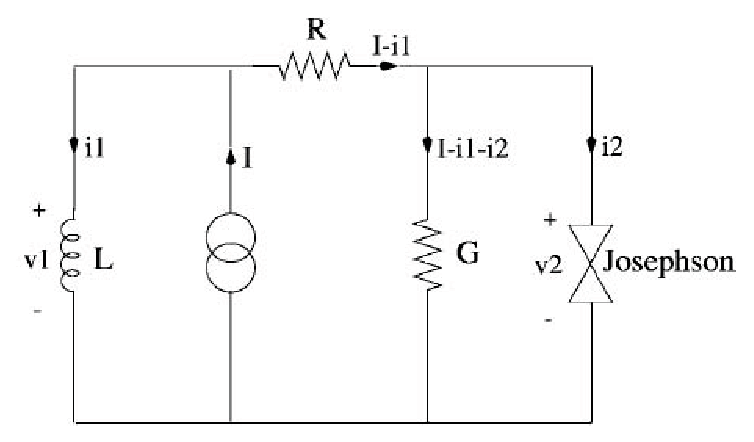
\includegraphics[scale = 0.6]{Josephson-junction}
	\caption{Electric circuit with Josephson junction, \cite{Ria04}}
	\label{josephson junction}
\end{figure}
%	
It is important to note that we will consider nonlinear instead of linear resistance, inductance and conductance as in \cite{Ria04}, and hence, 
we see that for the inductance $i_1 = i_L(L,\phi_1)$, for the resistance $v_R=v_R(R,i_1)$, and for the conductance $i_G=i_G(G,v_2)$.
Therefore, we obtain the following system, which completely describes the behavior of this circuit. 
%
\begin{subequations}
\begin{alignat}{4}
\label{5.5.1} \dot{\phi}_1 &= v_1, \\
\label{5.5.2} \dot{\phi}_2 &= v_2, \\ 
\label{5.5.3} i_1 &= i_L(L, \phi_1), \\ 
\label{5.5.4} i_2 &= I_0 \sin(k\phi_2), \\
\label{5.5.5} 0 &= v_1 - v_R(R, i_1) + v_2, \\
\label{5.5.6} 0 &= - i_G(G,v_2) + I - i_1 - i_2.
\end{alignat}
\end{subequations}
%
From \eqref{5.5.3}-\eqref{5.5.6} we obtain an explicit form of $v_1$ in terms of $\phi_1$, $i_1$ and $v_2$, so we can compress the system to obtain
%
\begin{subequations}\label{eq5.5}
\begin{alignat}{4}
\dot{\phi}_1 &= v_R(R,i_L(L,\phi_1)) + v_2, \\
\dot{\phi}_2 &= v_2, \\
i_1 &= i_L(L,\phi_1), \\ 
0   &= - i_G(G,v_2) + I - i_L(L,\phi_1) - I_0 \sin(k\phi_2). 
\end{alignat}
\end{subequations}
%
The linearized version of this system along equilibrium points defined by $v_2=0$, $i_1=I$, $\phi_1=LI$, $\phi_2=n\pi/k$, reads
%
\begin{align*}\label{eq5.6}
\dot{\phi}_1 &= RI - (R/L) \phi_1 + v_2, \\
\dot{\phi}_2 &= v_2, \\
i_1 &= \phi_1/L , \\ 
0 &= - G v_2 + I - \phi_1/L - I_0 \sin(k\phi_2),
\end{align*}
%
will have a positive eigenvalue and a negative one  (e.g. \cite{Ria04}). Hence, it admits exponential dichotomy for any odd number $n$. 
Thus, for $\vphi$-Lipschitz function $v_R$ and contraction mapping $i_G$, we obtain a stable manifold for \eqref{eq5.5}.
\end{example}
%
%%%%%%%%%%%%%%%%%%%%%%%%%%%%%%%%%%%%%%%%%%%%%%%%%%%%%%%%%%%%%%%%%%%%%%%%%%%%%%%%%%%%%%%%%%%%%%%%%%%%%%%%%%%%%%%%%%%%%%%%%%%%%%%%%%%%
%\subsection*{Acknowledgment}
%The authors would like to thank anonymous referees for his/her valuable
%comments and remarks that improved the paper.

%============================================================================
%\bibliographystyle{alpha}
\bibliographystyle{plain}
\bibliography{Huy_Phi_2019}

\end{document}

\begin{example}\label{exam0.2}{\rm
		The dynamical behavior of a system in fluid mechanics and turbulence modeling  is often described by
		the incompressible Navier-Stokes equation on an open, bounded domain $\Omega \subset \r^k$, $k=2$ or $3$, of the form
		%
		\begin{eqnarray*}
			\frac{\partial u}{\partial t} - \nu \De u + \nab p + (u\cdot \nab )u &=& F(t,u), \\
			\nab \cdot u &=& g(t,u),
		\end{eqnarray*}
		%
		where $\nu>0$ is the viscosity, $u=u(t,\xi)$ is the velocity field which is a function of the time $t$ and the position $\xi$, $p$ is the pressure, $f$ is the external force.
		Furthermore, we does not consider only the divergence-free case (i.e., $g\equiv 0$), due to many reasons from both analytical and numerical viewpoints. 
		%
		The first reason is that a nonzero $g$ may appear in generalized Navier-Stokes model of fluid structure interactions or in control framework, \cite{Ray10}. 
		%
		Secondly, from a numerical viewpoint, semi-discretization of flows with nonzero Dirichlet boundary conditions may lead to artificial non-zero $g$, \cite[]{AltH18}. Furthermore, to measure the complexity in the solution procedure, it is important to understand the smoothness requirement of the right-hand side appear within the solution. This is of importance also in the case $g=0$, since inexact solvers lead to errors that act like a nonsmooth inhomogeneity. 
		
		Then, discretizing the space variable by finite difference, finite volumes, or finite element methods \cite{GroR07}, one obtains a differential-algebraic system of the following form.
		%
		\begin{align*}
		M \dot{U} + (K+N(U)) \ U + C P &= F(U,P), \\
		C^TU &= g(U,P), 
		\end{align*}
		%
		where $U(t)$, $P(t)$ approximate the velocity $u(t,\xi)$ and the pressure $p(t,\xi)$, respectively. Here the leading matrix $M$ is either an identity matrix or a symmetric positive definite matrix depending on the spatial discretization scheme. Furthermore, the matrix $C^T M^{-1} \left( C - \dfrac{\partial f}{\partial P} \right)$ is nonsingular. Using linearization around a trajectory, we then obtain a system of the form \eqref{eq1}. Nevertheless, it is well-known, e.g. \cite{AltH18}, that the differentiation index of this system is two, and hence, it is not strangeness-free. Thus, one need to transform it first to obtain a strangeness-free DAE below.
		%
		\begin{align}
		M \dot{U} + (K+N(U)) \ U + C P &= F(U,P), \notag \\
		C^TM^{-1}C \ P - C^TM^{-1} ( F-(K+N(U)) \ U ) - g(U,P) &= 0 \ .
		\end{align}
		%
	}
\end{example}
%
